
\documentclass[12pt]{amsart}
\usepackage{geometry} % see geometry.pdf on how to lay out the page. There's lots.
\geometry{a4paper} % or letter or a5paper or ... etc
% \geometry{landscape} % rotated page geometry
\usepackage{url}
\usepackage{amsthm}
\usepackage{listings}
\usepackage{graphicx}
 \lstset{
         basicstyle=\footnotesize\ttfamily, % Standardschrift
         numbers=left,               % Ort der Zeilennummern
         numberstyle=\tiny,          % Stil der Zeilennummern
}

% See the ``Article customise'' template for come common customisations

   % The amssymb package provides \mathbb and other
   % math symbols.  The amsmath package provides sophisticated math
   % constructions.  The amsthm package provides \theoremstyle and
   % the \proof environment.
   %
   % The amsmath and amsthm packages are automatically activated by
   % \documentclass{amsart}, so there is no need to activate them here.

      \usepackage{amssymb}

   % Next we use \newtheorem to specify our theorem-like environments
   % (theorem, definition, etc.) and how to display and number them.
   %
   % Note: The \theoremstyle declarations affect the appearance of the
   % Theorems, Definitions, etc.

      \theoremstyle{plain}
      \newtheorem{theorem}{Theorem}[section]
      \newtheorem{lemma}[theorem]{Lemma}
      \newtheorem{corollary}[theorem]{Corollary}
      
      \theoremstyle{definition}
      \newtheorem{definition}[theorem]{Definition}
      
      \theoremstyle{remark}
      \newtheorem{remark}[theorem]{Remark}

   % The preamble is also a good place to define new commands and macros.
   % This part of the preamble is strictly optional according to your taste.

      \newcommand{\R}{{\mathbb R}}
      \newcommand{\nil}{\varnothing}

   % The following mysterious maneuver gets rid of AMS junk at the top
   % and bottom of the first page.
   
      \makeatletter
      \def\@setcopyright{}
      \def\serieslogo@{}
      \makeatother


\title{Suitability of the Teachspin muon lifetime device for testing QTD}
\author{Howard A. Landman}
\date{} % delete this line to display the current date

%%% BEGIN DOCUMENT
\begin{document}

\maketitle
\tableofcontents

\section{Introduction}
D. Apsel\cite{Apsel1978,Apsel1979,Apsel1981} and I\cite{Landman2012}, by entirely different methods,
both reached theories that predict the lifetime of an unstable particle can be altered by changing its energy.
I call this effect Quantum Time Dilation (QTD).
In particular, both of us predict that muon lifetime will be altered by an electrostatic potential to the extent of about 1\% per 1.05 MV.
This is clearly a testable assertion, but is sufficiently outside the mainstream of current physics research that it could be difficult to obtain funding from the usual sources to test it.
In the hope of keeping the cost of testing as low as possible,
I explore whether an inexpensive commercial student-grade muon lifetime apparatus can,
or can be modified to, provide a sufficiently accurate measure of muon lifetime to conclusively falsify or confirm these theories.

\section{The Teachspin device}
The Teachspin muon lifetime device\cite{Coan2006,Teachspin} is self-contained
except for needing an electrical outlet
and an external (Windows or Linux) computer to store and display data and run the user interface software.
It has three main components.
\subsection{The scintillator cylinder}
The primary detector comprises a solid transparent cylinder of scintillator-doped polyvinyltoluene,
a single photo-multiplier tube (PMT),
a high-voltage power supply for the PMT,
and an amplifier that converts the PMT current output to a voltage signal.
These are all contained in a light-tight aluminum shell
which keeps out external photons that could cause experimental noise or even damage the PMT,
and also keeps the high PMT voltage safely away from users.
The shell also includes an LED circuit for creating artificial light pulses to test the PMT independently of particles,
and some control knobs for the LED and the PMT.
I did not use the LED feature.

Charged cosmic ray particles, mostly muons, strike the cylinder and can generate photons in the scintillator.
Since cosmic rays have very high momenta (up to about 4 GeV/c)
and the cylinder is relatively small with low stopping power
(the manual says 120 MeV/c; our simulations using SRIM/TRIM software\cite{SRIM} gave about 62-70 MeV/c),
most (about 97\%) of the particles pass through the scintillator without stopping.

\subsection{The discriminator and counter}
Most of the active electronics is contained in a separate chassis.
It includes a discriminator circuit with adjustable threshold,
that can be tuned to reject pulses below the threshold.
This produces an amplified "digital" pulse if the input "analog" pulse exceeds the threshold.
The digital pulse has fixed height, but its width varies with the width of the analog pulse.

The digital pulse is then fed into an FPGA, which starts a lifetime count if one isn't already running.
Since the FPGA runs on a 50 MHz (20 nS) clock,
it is incapable of distinguishing times any shorter than that.
The count runs for 1000 clock cycles (20 $\mu$S);
if a second pulse is seen in that time, it is counted as a decay event, otherwise it is counted as a transit event.

Once a second, the number of events in the last second is written out, along with any decay events.
Each decay event, and each event summary, is communicated via USB to the computer.

\subsection{Computer and software}
Software running on the host computer writes one line of text to the data file
for each decay event, and one for each event summary.
These are the only kinds of data in the files.

For summary records, the number of events seen is recorded, followed by a timestamp.
Consecutive timestamps differ by one.

For decay events, the time between pulses in nS is written,
and is always a multiple of 20 since it is computed by multiplying the raw count from the FPGA by the nominal clock period.
It is also followed by a timestamp (number of seconds since some arbitrary starting date).
Typically there are many seconds between decay events, although it is possible to have more than one in the same second.

For the most part, in my analysis I only use the decay event records.
I did however perform some "sanity checks" on the summary records,
with interesting results described below.

\subsection{Alternatives}
Similar experiments, using different equipment,
are routinely performed at CalTech\cite{CaltechMuon}, UC Berkeley\cite{Berkeley2012}, U Mich\cite{Akerlof2009}, U Minnesota\cite{Hansen2001}, and elsewhere.
Most of these use scintillators far too large for our purposes.
However, the lab notes describe equipment configurations for discrimination, timing and counting
that could be useful.

There are other inexpensive detector options,
including several do-it-yourself ones\cite{CRDetectors},
but I don't analyze them in detail here.
The FermiLab detector\cite{FermiLabDetector} seems the most promising of these,
as it can do muon lifetime experiments and be powered by batteries.

\section{Statistical preliminaries: exponential and geometric distributions}

Before getting into the many sources of experimental noise and error,
it will be worthwhile to analyze the situation where no such problems exist.
For this purpose, we assume that we can measure a decay to infinite precision
and that all events seen are real decays.
We may also assume that the desired effect exists
and can be precisely controlled,
so that we may alter the muon lifetime at will.
Then, we are left with the purely statistical problem
of estimating the muon lifetime from a finite sample of decay events.

Even in the absence of an kind of experimental error,
the inherently random nature of exponential decay introduces a source of variance which cannot be removed.
Given the importance and simplicity of the exponential distribution,
the question of how much data must be sampled has been studied extensively.
Computing this will give us a hard lower bound for the actual experiment, as truncation, binning, noise and error can only increase this number.

Not everything in this section is actually used in the data analysis that follows later.
Topics that aren't are included in the hope that they may prove useful in related experiments.

\subsection{Maximum Likelihood Estimate and its confidence intervals}

The maximum likelihood estimate $\hat{\tau}$ for the lifetime is just the average of all the measured decay times,
\[ \hat{\tau} = \frac{1}{n}\sum_{k=1}^{n}t_k \]
with an exact $100(1-\alpha)\%$ confidence interval given by\cite{wiki_exponential}
\[ \frac{2n\hat{\tau}}{\chi^2_{1-\alpha/2,2n}} < \tau < \frac{2n\hat{\tau}}{\chi^2_{\alpha/2,2n}} \]

Using an online $\chi^2$ calculator\footnote{Using the "Calculate $X^2$ from probability $Q$ and $d$" function at \url{http://www.fourmilab.ch/rpkp/experiments/analysis/chiCalc.html} and iterating on $d$ until it converges to the desired value for $\chi^2$. This algorithm only appears to be numerically stable to about 7 decimal places, so any digits beyond that may not be meaningful.} we get Table 1.

\begin{table}[hbtp]
    \caption{Events $n$ needed to get confidence $(1-\alpha)$ at given $\chi^2$}
    \begin{tabular}{|r|r|r|r|r|r|}
        \hline
        ~                                                  & $\alpha=.02$ & $\alpha=.01$ & $\alpha=.005$ & $\alpha=.002$ & $\alpha=.001$  \\
        \hline
        5.25 MV ($\frac{\chi^2_{\alpha/2,2n}}{2n}=1.050$)  & 3459         & 4446         & 5457          & 6820          & 7866           \\ 
        2.10 MV ($\frac{\chi^2_{\alpha/2,2n}}{2n}=1.020$)  & 21303        & 27353        & 33549         & 41903         & 48316          \\ 
        1.05 MV ($\frac{\chi^2_{\alpha/2,2n}}{2n}=1.010$)  & 84786        & 108825       & 133447        & 166644        & 192125         \\ 
        525 kV ($\frac{\chi^2_{\alpha/2,2n}}{2n}=1.005$)   & 338287       & 434124       & 532287        & 664630        & 766205         \\ 
        210 kV ($\frac{\chi^2_{\alpha/2,2n}}{2n}=1.002$)   & 2111068      & 2708846      & 3321111       & 4146496       & 4779886        \\ 
        105 kV ($\frac{\chi^2_{\alpha/2,2n}}{2n}=1.001$)   & 8439886      & 10829342     & 13276595      & 16575156      & 19105704       \\
        \hline
    \end{tabular}
\end{table}

This table can be read in two ways.
First, it tells us how many data points we need to know the true lifetime to within a certain error with a given level of confidence.
For example, to know the lifetime to within 0.1\% with 98\% confidence, we need 8439886 events (first column, last row).
This is a two-tailed test, as our estimate could be either too high or too low.
For this purpose, we read the $\chi^2$ but ignore the voltage.

We can also use it to determine the number of events needed (assuming the theory is true) to produce a result with any given degree of unlikeliness in the null hypothesis (that there is no effect).
This varies with the voltage of the VDGG, since higher voltages are predicted to produce stronger effects which are easier to distinguish from random noise.
Thus, we can read it as the number of events required, at a given voltage, to produce data making the null hypothesis as unlikely as desired.
(If we pick a single direction, we have a one-tailed test and so the statistical significance level is actually $\alpha/2$.)

%Very roughly, the number of data points required goes down as $1/V^2$ and up as $-\log(\alpha)$ (guessing, need to check).
Given that higher voltages should require many fewer events, it seems desirable to get as large a voltage as practicable, so as to reduce the data requirements.
However, larger VDGGs are more expensive.
Very roughly, the sphere diameter needs to be at least 1 mm per kV (= 1 m per MV),
and the mass (and hence material cost) of the VDGG goes up as at least the cube of this.

\subsection{Sequential Probability Ratio Test}

When one is only trying to distinguish two hypotheses $H_0$ and $H_1$,
and is collecting data slowly over time,
a log-likelihood approach leads directly to the Sequential Probability Ratio Test (SPRT)\footnote{see
Gold \& Shadlen\cite{Gold2007} pages 538-542 for a nice brief exposition, particularly the sidebar on page 541.}
of Signal Detection Theory.
To the $i$th piece of evidence $e_i$ (in this case, a measured decay time) we assign a weight
\[ w_i = \log\frac{P(e_i|H_1)}{P(e_i|H_0)} \]
and our decision variable $y$, the log-likelihood after $n$ samples, is given by the simple sum
\[ y_n = \log\frac{P(e_1,e_2,...,e_n|H_1)}{P(e_1,e_2,...,e_n|H_0)} = \sum_{i=1}^n\log\frac{P(e_i|H_1)}{P(e_i|H_0)} = \sum_{i=1}^nw_i \]
The termination criterion is that we stop and say $H_1$ is true if $y_n \ge \log\frac{1-\alpha}{\alpha}$,
and we stop and say $H_0$ is true if $y_n \le \log\frac{\beta}{1-\beta}$,
and otherwise we continue to collect data.
Here $\alpha$ is the acceptable probability that we falsely conclude $H_1$ is true,
and $\beta$ the acceptable probability that we falsely conclude $H_0$ is true.

For the special case of two exponential distribution hypotheses differing only in their lifetime parameter,
($\frac{1}{\tau_0}e^{-t/\tau_0}$ versus $\frac{1}{\tau_1}e^{-t/\tau_1}$),
we have that
\[ P(e_i|H_0) = \frac{1}{\tau_0}e^{-t_i/\tau_0} \]
\[ P(e_i|H_1) = \frac{1}{\tau_1}e^{-t_i/\tau_1} \]
\[ w_i = w(t_i) = \log\frac{P(e_i|H_1)}{P(e_i|H_0)} = \log(\frac{1}{\tau_1}e^{-t_i/\tau_1}) - \log(\frac{1}{\tau_0}e^{-t_i/\tau_0}) \]
\[ = \frac{-t_i}{\tau_1} - \log(\tau_1) - \frac{-t_i}{\tau_0} + \log(\tau_0) \]
\[ = \left(\log(\tau_0) - \log(\tau_1)\right) + t_i(\frac{1}{\tau_0} - \frac{1}{\tau_1}) \]
%\begin{align*}
%& w_i = w(t_i) = \log\frac{P(e_i|H_1)}{P(e_i|H_0)} = \log(\frac{1}{\tau_1}e^{-t_i/\tau_1}) - \log(\frac{1}{\tau_0}e^{-t_i/\tau_0}) \\
%& = \frac{-t_i}{\tau_1} - \log(\tau_1) - \frac{-t_i}{\tau_0} + \log(\tau_0) \\
%& = \left(\log(\tau_0) - \log(\tau_1)\right) + t_i(\frac{1}{\tau_0} - \frac{1}{\tau_1})
%\end{align*}
The expected weight if $H_1$ is true would then be
\[ \langle w|H_1 \rangle = \int_0^{\infty} P(t)w(t)dt \]
\[ = \int_0^{\infty} \frac{1}{\tau_1}e^{-t_i/\tau_1} \left( \left(\log(\tau_0) - \log(\tau_1)\right) + t_i(\frac{1}{\tau_0} - \frac{1}{\tau_1}) \right) \]
\[ = \left(\log(\tau_0) - \log(\tau_1)\right)\int_0^{\infty} \frac{1}{\tau_1}e^{-t/\tau_1} dt + (\frac{1}{\tau_0} - \frac{1}{\tau_1}) \int_0^{\infty} \frac{1}{\tau_1} t e^{-t/\tau_1} dt \]
But the first integral is just 1 and the second integral just gives the expected value of $t$ over the entire distribution, which we know is $\tau_1$, so
\[ \langle w|H_1 \rangle =  \left(\log(\tau_0) - \log(\tau_1)\right) + (\frac{\tau_1}{\tau_0} - 1) \]

If we are able to change the muon lifetime by a fraction $\delta$, so that $\tau_1 = (1+\delta)\tau_0$, then
\[ \langle w|H_1 \rangle =  \left(\log(\tau_0) - \log((1+\delta)\tau_0)\right) + (\frac{(1+\delta)\tau_0}{\tau_0} - 1) = \delta - \log(1+\delta) \]
For $\delta=0.01$, which is what we would predict for a voltage of 1.05MV, we get
\[ \langle w|H_{1.01\tau_0} \rangle = 0.01 - 0.009950331 = 0.000049669 \]
This can be used to directly calculate the expected number of events needed to achieve any given likelihood ratio.
For example, if we want $H_1$ to be 1000 times more likely than $H_0$, we need about
\[ \frac{\log(1000)}{\langle w|H_1 \rangle} = \frac{6.907755}{0.000049669} = 139075 \pm 373 \]
decay events, where $373 \approx \sqrt{139075}$ is an estimate of the standard deviation of this number.
This is roughly comparable to the estimate 166644 given in the $\chi^2=1.01, \alpha=.002$ entry of Table 1.

\subsection{Fisher Information analysis}

We can also analyze this in terms of Fisher Information.
FI is mostly useful through the Cramer-Rao inequality
\[ (\Delta \tau)^2 \ge \frac{1}{I(\tau)} \]
in which the inverse of the Fisher Information gives a lower bound on the variance of our estimate of the lifetime $\tau$.

The FI for our purposes measures the amount of information that a single decay time $t$ carries about the unknown lifetime parameter $\tau$ upon which the probability of $t$ depends.
It is defined as the expectation of the square of the partial derivative with respect to the parameter of the log-likelihood function.
\[ I(\tau) \equiv E\left[ \left( \frac{\partial}{\partial\tau} \log f(t;\tau) \right)^2 \bigg| \tau \right] = E\left[ \left( \frac{\partial}{\partial\tau} \log \left(\frac{1}{\tau}e^{-t/\tau}\right) \right)^2 \bigg| \tau \right] \]
\[ = E\left[ \left( \frac{\partial}{\partial\tau} \left(\frac{-t}{\tau} -\log(\tau)\right) \right)^2 \bigg| \tau \right] = E\left[ \left( \frac{t}{\tau^2} - \frac{1}{\tau} \right)^2 | \tau \right] = \frac{1}{\tau^4} E\left[ (t-\tau)^2 \big| \tau \right] \]
But this last expectation is just the variance of $t$, which is $\tau^2$, so the FI for a single decay event is
\[ I(\tau) = \frac{1}{\tau^2} \]
and for $n$ decay events is just
\[ I(\tau) = \frac{n}{\tau^2} \]
so that 
\[ (\Delta \tau)^2 \ge \frac{1}{I(\tau)} = \frac{\tau^2}{n} \]
or
\[ \frac{\Delta \tau}{\tau} \ge \frac{1}{\sqrt{n}} \]
If we assume approximately Gaussian error in $\tau$ for $n$ large,
we can use this to estimate the minimum number of events required
to know $tau$ with a standard deviation $\sigma \equiv \Delta\tau < \alpha\tau$ as
\[ n \ge \frac{1}{\alpha^2} \]
From this we can see that $\alpha=.001$ gives $n \ge 1000000$.
This is not exactly comparable to the numbers calculated above,
since for $H_1$ and $H_0$ differing by 1\% it would separate the two hypotheses by 10$\sigma$.

If we apply this to the latest MuLan muon lifetime number $2.197019\pm0.000021$ $\mu$S\cite{MuLan2007},
we get $n \ge 10945334436$,
implying that it should have taken a {\em minimum} of about 11 billion muon decay events to achieve this accuracy,
even in the complete absence of any experimental error.

%\section{Exponential distribution with uniform noise}

%(NOTE THIS SECTION IS NOT RIGHT YET!)

%Now that we fully understand the behavior of a pure exponential distribution,
%and before we start considering the many sources of experimental error,
%let's briefly look at the pure exponential with a pure uniform noise source added.
%The key observation here is that,
%if we are only concerned with the {\em first} event,
%then the time to that event for a uniform distribution is in fact exponentially distributed!
%Thus (if we ignore all following events)
%we can characterize the rate parameter $\nu$ of the noise (in events per second)
%and the rate parameter $\lambda = 1/\tau$ of the decay,
%and simply add them to get the total rate.
%For $N$ starting particles, this gives us a density of events at time $t$ of
%\[ f(t;\tau,N,\nu) = Nf(t;\tau) + \nu = \frac{N}{\tau} e^{-t/\tau} + \nu \]
%Note that this is {\em not} a probability distribution, since the $\nu$ part is not normalizable.
%However if we truncate this to any finite window,
%it becomes a perfectly fine distribution and easy to normalize.

%\subsection{Fisher Information analysis}

%Here it easier to use the chain rule form of Fisher Information by noting that
%\[ \frac{\partial}{\partial\tau}\log f(t;\tau,N,\nu) = \frac{\frac{\partial}{\partial\tau} f(t;\tau,N,\nu)}{f(t;\tau,N,\nu)} 
%= \frac{N \frac{\partial}{\partial\tau} f(t;\tau,1,0)}{f(t;\tau,N,\nu)} \]
%since $\partial\nu / \partial\tau = 0$ and $N$ can be pulled outside the derivative.
%This is similar to the formula {\em without} noise,
%except for the $\nu$ term in the denominator.
%Thus the noise acts to dilute or reduce the information obtained, in a ratio of
%\[ \frac{I(\tau,N,\nu)}{I(\tau,N,0)} = \frac{f(t;\tau,N,0)}{f(t;\tau,N,\nu)} \]

%This gives us
%\[ I(\tau;N,\nu)  = E\left[ \left( \frac{N\frac{\partial}{\partial\tau} \left(\frac{1}{\tau} e^{-t/\tau} \right)}{\frac{N}{\tau} e^{-t/\tau} + \nu} \right)^2 \bigg| \tau \right] \]
%\[ = E\left[ \left( \frac{\frac{\partial}{\partial\tau} \left(\frac{1}{\tau} e^{-t/\tau} + \nu \right)}{\frac{N}{\tau} e^{-t/\tau} + \nu} \right)^2 \bigg| \tau \right]
%  = \frac{1}{\tau^4} E\left[ (t-\tau)^2 \big| \tau \right] \]
%%But this last expectation is just the variance of $t$, which is $\tau^2$, so the FI for a single decay event is
%%\[ I(\tau) = \frac{1}{\tau^2} \]
%%and for $n$ decay events is just
%%\[ I(\tau) = \frac{n}{\tau^2} \]
%%so that 
%%\[ (\Delta \tau)^2 \ge \frac{1}{I(\tau)} = \frac{\tau^2}{n} \]
%%or
%%\[ \frac{\Delta \tau}{\tau} \ge \frac{1}{\sqrt{n}} \]

%\section{Sources of error in the estimation of muon lifetime}

%\subsection{Randomness of decay}

%However, even an inexpensive educational VDGG can reach 500 kV, so that we are unlikely to have to go below the fourth row.
%Achieving .001 significance even at that level only requires about 766K events.

%We also know that "sequential sampling from an exponential population is essentially equivalent to observing a Poisson process"\cite{Sayyad1969}
%and that the variance of a Poisson process with parameter $\lambda$ is itself $\lambda$.
%(Note that $\lambda = 1/\tau$, where $\tau$ is the $1/e$ lifetime.)
%That is, for any given $\lambda$, the number of decays seen in each bin is Poisson-distributed.

%Assuming we are measuring a muon lifetime $\tau$ that has been altered by 1\%, and wish to distinguish it from the unaltered one $\tau_0$ at a significance level $\alpha$,
%we need the relative likelihood of the experimental evidence under the default hypothesis $H_{\tau_0}$ versus the time-altered hypothesis $H_\tau$ to be less than $\alpha$.
%There are several ways to approach estimating how much data this requires.

\subsection{Truncation of distribution}

It is traditional to truncate the exponential distribution on the right;
the Teachspin software does this by default at no more than 20 $\mu$S (about 9 lifetimes).
This is done both because we cannot wait forever for any single muon to decay,
and because after some time any "decay" event seen is much more likely to be noise than an actual decay.
However, it is rare that this truncation is treated exactly.

In this subsection we continue to ignore the noise issue,
but focus entirely on the problem of estimating the true distribution mean from a truncated sampling procedure.
This problem has been solved analytically by Al-Athari\cite{Al-Athari2008};
most of what follows is adapted from his paper.

Let the length of the sampling interval be $b$.
If our complete distribution is
\[ \frac{1}{\tau} e^{-t/\tau} \]
with mean $\tau$, the truncated distribution has mean
\[ \tau' = \tau - \frac{b}{e^{b/\tau} - 1} \]
where the second term essentially subtracts off the mean of the truncated portion,
weighted by the probability that a sample from the full distribution would be truncated.

Especially for large sample size $n$, we would expect the sample mean $\bar{t}$ to be less than $b/2$,
but there is some probability that this will not be true.
If it isn't, then no maximum likelihood estimator exists.
However, the chance of this occurring rapidly approaches 0 as $n\rightarrow\infty$.

The likelihood function is
\[ \frac{e^{-n\bar{t}/\tau}}{\tau^n(1-e^{-b/\tau})^n} \]
Maximizing this (or more usually its log) gives the MLE $\hat{\tau}$ for $\tau$.
(Al-Athari actually finds the MLE for $\theta = 1/\tau$,
but since he uses the log-likelihood,
the inversion becomes just a sign change and the MLE is the same either way.)
If $\bar{t} < b/2$ we are guaranteed that the MLE exists,
i.e. that the derivative of this is zero at some finite value.
(If $\bar{t} \ge b/2$, the MLE doesn't exist, but we can use $b/2$ as our estimate.
This is Al-Athari's Modified MLE (MMLE), and is equivalent to assuming a uniform distribution,
which is the limit of the exponential distribution as the lifetime goes infinite.)

Thus (skipping a few steps) we want to solve
\[ n ( \hat{\tau}' - \bar{t} ) = 0 \]
i.e. find the $\hat{\tau}'$ that correctly predicts the sample mean.
(In the full exponential case this is simply $\hat{\tau} = \bar{t}$.)
Since we know $n$ is not zero, we get $\hat{\tau}' = \bar{t}$.

Al-Athari stops here, but that doesn't give us a closed-form solution for $\hat{\tau}$ as a function of $b$ and $\bar{t}$.
Substituting back in, we get
\[ \hat{\tau}' = \hat{\tau} - \frac{b}{e^{b/\hat{\tau}} - 1} = \bar{t} \]
which can be solved numerically for $\hat{\tau}$ given $\bar{t}$ and $b$.
%\[ \hat{\tau} - \bar{t} = \frac{b}{e^{b/\hat{\tau}} - 1} \]
%\[ (e^{b/\hat{\tau}} - 1)(\hat{\tau} - \bar{t}) = b \]
%\[ e^{b/\hat{\tau}}\hat{\tau} - e^{b/\hat{\tau}}\bar{t} - \hat{\tau} + \bar{t} = b \]

\subsection{Binning and the geometric distribution}

The Teachspin timing FPGA operates on a 50 MHz (20 nS) clock $\pm$100 ppm.
Ignoring clock error for the moment,
what is the effect of putting decays into finite-width bins?

\subsubsection{Geometric distribution}

Binning converts the exponential distribution into a geometric distribution.
%(This is the only discrete distribution which is memoryless.)
If we number the bins starting at 0, the probability that a single muon will decay in bin $k$ is
\[ P(K=k) = (1-p)^kp \]
where $p$ is the probability that a muon will decay in 1 bin time if it has not decayed already.
For a given lifetime $\tau$ and bin width $b$, we have
\[ p = p(\tau,b) = \int_{t=0}^b \frac{1}{\tau}e^{-t/\tau} dt = -e^{-t/\tau}\bigg|_0^b = 1 - e^{-b/\tau} \]
For $\tau = 2031.79$ nS (our experimental result below), and $b = 20$ nS, this gives $p = 0.0097574$,
so for each bin there is about a 1\% chance that a muon will decay, and a 99\% chance it will survive.
The expected value is just
\[ \langle K \rangle = \frac{1}{p} \]
and the MLE for $p$ just the inverse of the sample mean
\[ \hat{p} = \frac{1}{\bar{K}} \]

Truncation of the geometric distribution has similar effects to truncation of the exponential distribution.
The probability that a muon which decays in one of the first $B$ bins will decay in bin $k$ is
\[ P(K=k) = \frac{(1-p)^kp}{1 - (1-p)^B} \]
which renormalizes the truncated distribution to have total probability 1.

\subsubsection{Bin offset}

The decays within a bin could of course have happened at any time during the bin window.
For very small bins, we expect that the average decay time within a bin will be slightly less than
the bin start time plus half the bin width,
since the exponential distribution is monotonic decreasing.
We can quantify this precisely using the truncated exponential analysis given above.
Let $\tau'(\tau,b)$ be the expected value of the decay time in a bin of width $b$.  Then
\[ \tau'(\tau,b) = \tau - \frac{b}{e^{b/\tau} - 1} \]
as before, except that we now expect $b/\tau$ to be fairly small.
For $\tau = 2031.79$ nS and $b = 20$ nS, this gives $\tau' = 9.9836$ nS,
which is (as expected) slightly less than 10 nS.
Thus, for an unbiased estimate with that $\tau$ and $b$, we should treat all the decays in the $k$th bin
(which spans 20$k$ to 20$(k+1)$ nS)
as if they decayed at 20$k$ + 9.9836 nS.

Failing to do this and instead using 10 nS would give a positive bias to our estimated $\tau$ of about 0.0164 nS,
or about +8 ppm.
This is small relative to the clock uncertainty of $\pm$100 ppm.

\subsection{Exponential and geometric decay are memoryless}

We note here in closing that a property unique to the exponential and geometric distributions is that they are {\em memoryless};
the probability of an event occurring does not depend on how long we have already waited for it to occur.
Another way of saying this is that they have a constant failure rate.
Because muon decay (like nuclear decay) follows an exponential decay pattern,
we do not need to be concerned with the history of the muon before it arrives in our apparatus.
Indeed, the entire experiment would not be possible without this property,
since we do not measure the {\em entire} lifetime of the muon from its creation in a pion decay while still traveling at nearly lightspeed,
but only its lifetime after coming to rest in our detector.


\section{Sources of Experimental Error}

Here are all the sources of error I can think of in the Teachspin experiment,
along with analyses of their effects and any ways of eliminating or compensating for them.

\subsection{Offset between stopping and decaying pulses}
The light in a stopping pulse is generated BEFORE the muon stops, while it is still moving.
The light in a decay pulse is generated AFTER the muon decays, mostly by the emitted electron.
Since the pulse detector works on the leading edge of both, that means it starts counting the stopping pulse too soon.
If the muon is still moving, there may be some SR time dilation that would lengthen its lifetime.

NET EFFECT: Should make measured lifetimes longer than actual ones.
Rough order of magnitude would be the width of the stopping pulse.
For my setup, the analog pulses were about 25-35 nS wide at the base, and about 4-20 nS wide at trigger level,
based on visual inspection of about a hundred pulses on a digital storage scope.
Thus we estimate a systematic bias of about $(4 + 20)/2 = 12$ nS and a $\sigma$ of no more than 8 nS for this ($\sigma^2 = 64$ nS$^2$).

SOLUTION: Discarding initial bins (see below) makes this problem go away for the stopping pulse.
For the decay pulse, we get a triggering offset of about 9 nS (from start of pulse to time of trigger) $\pm$8 nS.
We also have to add another 5.5$\pm$1.5 nS offset from the analog pulse to the digital pulse.
This gives us a total triggering correction and error of $\delta_{trig} = -14.5 \pm 9.5$ nS.

\subsection{Error due to variability in pulse size/shape}
% (2a stopping pulse, 2b decay pulse)
Since the discriminator circuit is tuned to a specific voltage level, and the leading edge has finite slope, and the size of the pulse may vary, we would expect a larger pulse to trigger slightly sooner than a smaller pulse.

NET EFFECT: Random errors in the time that the pulse is detected.
Min to max range would be somewhat less than half the typical pulse width
(soonest would be the point where the largest pulse triggers, latest would be near the middle (top) of a small pulse just barely able to trigger).
Based on the observations above, we estimate this to contribute $\sigma_p=4$ nS ($\sigma_p^2 = 16$ nS$^2$) for each pulse.

SOLUTION: Discarding initial bins removes this problem for the stopping pulse, but not for the decay pulse.

\subsection{Metastability of discriminator}
% (3a stopping pulse, 3b decay pulse)
Any time a circuit has to take an analog input and make a digital decision on it, there will be signals very close to the decision threshold that can cause the circuit to hang in a metastable intermediate state.  (This problem occurs most famously with flip-flops receiving data asynchronously to their clocks, but it can be caused by thresholds in voltage as well as in time.)  There is no theoretical upper bound to how long this hanging can occur; however, the probability of continued hanging decays exponentially with time (it is an unstable equilibrium like a pencil balancing on its point).  The exact behavior depends on circuit construction; a good circuit can make this problem very unlikely, at the cost of taking more time to make the decision.  I don't know yet what the details of the Teachspin discriminator are.

NET EFFECT: Until analyzed more closely,
we should assume that there may be occasional pulses which are effectively delayed by an entire clock cycle, or even (much more rarely) two.
Since this can happen on either pulse, it could lengthen or shrink the measured decay time.
Large and small pulses may behave differently;
if there is a difference in pulse sizes between stopping and decay pulses, we could get a net average offset, but if not the mean of this should be zero.
Although the magnitude of such an error would be on the order of $\pm10$ nS,
metastability events are very rare (1 in millions or billions), so the estimated $\sigma_{ms}$ here would be 0.1 nS or less.

\subsection{Digitization error of pulse time}
% (4a stopping pulse, 4b decay pulse)
I assume that the pulses are digitized to synchronize with a clock pulse that has 20 nS (the bin size) cycle time since the file data is reported in multiples of 20 nS.

NET EFFECT: This adds a random error which is roughly uniformly distributed over the 20 nS cycle time,
giving a systematic offset of approximately half the cycle time or 10 nS,
and adding a variance of approximately $\sigma_{dig}^2 = \frac{1}{12}(20\ nS)^2$ \cite{wikiUniform}
to a single event time.
If both stopping and decay pulses contribute this, the offsets cancel but the variances add.
For $n$ events, this variance scales linearly, so the standard deviation of the average scales as $1/\sqrt{n}$.

SOLUTION: Discarding initial bins removes this problem for the stopping pulse, but not for the decay pulse.
For either pulse, to zeroth order we can treat all decays in a bin as occurring at the center of the bin (+10 nS).
As noted earlier, a more exact correction can be computed if we know the decay time.
Since we use this number to compute the estimated decay time,
we would appear to be using circular reasoning;
however, since the effect of the decay time on the offset is small,
and the effect of the offset on the decay time is small,
in practice we can ``go around the circle'' a few times and get excellent convergence.
%IMPLEMENTATION: I currently use the zeroth order correction only (all decays are assumed to be at the center of their bin, i.e. 10 nS after the bin start for 20 nS bins).
%I plan to change this to the more exact number

IMPLEMENTATION:
Using the bin offset formula above plus the uniform approximation for variance, we take $\delta_{dig} = (\tau - \frac{b}{e^{b/\tau} - 1}) \pm \frac{10}{\sqrt{3n}}\ {\rm nS}$.
%However, bin offset is not needed when fitting to a geometric distribution.

\subsection{Inability to detect very fast decays}
Very fast decays may be difficult or impossible to detect.
Since the scintillator takes nanoseconds to emit all its light,
two pulses starting less than a few nanoseconds apart may appear to be one wide pulse.
There may also be issues throughout the analog circuitry, from the PMT to the discriminator;
each may require some time after emitting a pulse to recover and be ready for another one.
The recording computer, USB interface, and software may also impose limits.
Examination of a large output file with over 100K decay events shows zero decays in the 0 nS and 20 nS bins,
and a reduced number of decays in the 40 nS bin.
This implies that all decays shorter than about 40-50 nS are being lost.

NET EFFECT: Decays faster than some minimum time are lost.
Fitting to this data will give wrong answers.

SOLUTION: Fortunately, exponential decay is memoryless.  We can simply discard the first few bins to solve this problem.
Doing so also fixes many of the above problems.
It also has the effect of synchronizing all the muon decay start times with the beginning of the first undiscarded bin.

IMPLEMENTATION: My analysis software currently discards the first 3 bins (all decays marked as 40 nS or less).
This loses about 0.1\% of the data, which is acceptable.

\subsection{Clock jitter and drift}
The clock driving the bin sampling is not perfect, but will have some jitter.
It may also drift slightly over time due to temperature, circuit aging, power supply variation, or other causes.
For any reasonably good crystal oscillator, this will probably be much smaller than some other sources of error listed here and so negligible, but it is not zero.
Teachspin claims its clock is accurate to $\pm$100 ppm.
This could be measured by a device with a more accurate clock,
but for this report we simply assume that the clock period may both have a fixed offset of $\pm 2$ pS (100 ppm of 20 nS)
and a uniformly-distributed random jitter of the same magnitude, contributing $\frac{1}{12}(4\ {\rm pS})^2$ variance to individual decay times.
This jitter is so much smaller than the digitization error above that we ignore it.

NET EFFECT: We are left with a $\delta_{clock} = \pm10^{-4}\tau$ from our uncertainty about the actual clock period.

\subsection{False decay noise due to separate transit events close together}
This is probably the largest and most serious noise problem in the experiment.

NET EFFECT: If we assume that the transits are random, then the first transit has a uniform probability over time and the second one has the same distribution, so the probability of a false decay event from two transits is proportional to the decay window size times the square of the transit probability.

SOLUTIONS: Given the power of 2, the easiest way to reduce this noise would be to reduce transit events.  Cutting them down by a factor of 10 would reduce the false decay from this cause by a factor of 100.  One approach of course is to use a muon beam with momentum tuned to mostly stop in the detector, i.e., to increase the number of true decay events relative to the false ones.  Staying with cosmogenic muons only, detector paddles above and below the main scintillator could give signals that would allow us to detect and filter out many transit events.

It is also possible to estimate the mean number of false decays per bin and to "subtract that out" of the data in various ways.  However, this still leaves residual errors from (a) the error in estimating the mean, and (b) the variation about the mean.  An alternate statistical approach would be to leave in all the decay events (true and false), but estimate the probability that each one is true (which will depend on the bin) and weight them accordingly.  This is particularly simple in the Bayesian approach, where the log (relative) probability of the (true) event is simply added to the log (relative) likelihood of the hypothesis: we can just multiply that log event probability by the probability that the event is true and add that instead.

IMPLEMENTATION: We fit a model which has noise level as a parameter.
Both errors in fitting the average noise level, and variance from the noise, should contribute error to our lifetime estimate,
but quantifying these errors is not trivial.
It can be estimated from Monte Carlo simulation, but we haven't done that.
 
\subsection{Correlated noise}

In the previous subsection we assumed that the background noise is independent,
i.e.\ that the probability of a transit event is not correlated with other transit events.
There could be cases where this is not true.
For example, a highly energetic cosmic ray hitting part of the building structure
could generate a shower of secondary particles
and thus cause a cluster of transit events.

Since these particles would mostly still be traveling at close to lightspeed,
and light travels about a foot per nanosecond,
the time skew between two particles (in nS)
would be roughly the length difference of their paths to the detector (in feet).
We expect that most of these clusters of events would spread only a few nS,
and thus are being filtered out both by the inability of the device to measure short delays
and by our discarding of the first three 20 nS bins.
Thus, only skews of greater than 60 nS (implying either a delta-path-length of over 60 feet,
or one particle moving much slower than lightspeed)
would be able to cause false decay events.
These seem sufficiently unlikely that we can ignore them.

\subsection{Transit Time Spread in PMT}

"The delay between the absorption of a photon at the photocathode and the output pulse from the anode of a PMT
varies from photon to photon.
The effect is called 'transit time spread' or TTS.
There are three major TTS components in conventional PMTs and MCP PMTs - the emission at the photocathode, the multiplication process in the dynode system or microchannel plate, and the timing jitter of the subsequent electronics."\cite{Becker2003}

NET EFFECT:
Even in fairly slow PMTs. the TTS is rarely greater than 100 pS.
This is small relative to some of the other sources of error we have considered, but we include a $\sigma_{tts}=\pm0.1$ nS for completeness.

\subsection{Afterpulsing}

"Most detectors have an increased probability to produce a dark count pulse in a time interval of some 100 nS to some $\mu$S after the detection of a photon."\cite{Becker2003}
If we were doing single-photon detection,
this would be interpreted as a (false) decay event if it occurred within the decay window.
In this sense, afterpulsing is similar to background noise from transit events.
However, the background noise is uncorrelated, while afterpulsing is highly correlated.
Also, since we are looking for a large burst of photons rather than single photons,
a single-photon-sized event would not normally trigger the pulse detector
(our detector threshold (about 14 mV) was set well above the dark noise level of the PMT (about 1 mV)).

NET EFFECT: We expect afterpulsing to at worst slightly raise the dark noise level,
and thus not be a serious source of false decay events by itself.
However, it might slightly alter the pulse height threshold for decays at the afterpulse time.
This could have the effect of slightly increasing the number of decay events seen around the afterpulse time,
and hence slightly biasing the decay lifetime collection.

Since we have so far no details about the afterpulse behavior of the specific PMT used,
it is difficult to estimate the magnitude of any such error.

\subsection{Binomial sampling noise of $\mu^+ / \mu^-$ mixture}
All of the above would apply even if all the muons were a single type.
However, cosmogenic muons are are a mixture of muons ($\mu^-$) and antimuons ($\mu^+$)
with a slight excess of antimuons.
Values for the ratio of $\mu^+/\mu^-$ (the "charge ratio" $r$) in the literature vary from 1.08 to 1.3.

The CPT Theorem plus the assumption of EM-gauge invariance (as in the Standard Model)
would require that these have identical masses and lifetimes in vacuum,
but in matter their lifetimes differ because $\mu^-$ have an additional decay mode
of being captured by an atomic nucleus.
The best current lifetime numbers are $\tau_+ = 2197.019\pm0.021$ nS\cite{MuLan2007} for $\mu^+$ in vacuum
and $\tau_- = 2043\pm3$ nS for $\mu^-$ in carbon.

The lifetime measured in the Teachspin device is a weighted average of these two numbers,
with the weights given by the actual numbers of $\mu^+$ and $\mu^-$ detected.
However, we don't know these actual numbers, and they will vary from data set to data set.
So the expected mix of muons and antimuons will have a binomial distribution

\[ f(n_+;n,p) = \binom{n}{n_+} p^{n_+}(1-p)^{n_-} \]

where $n$ is the total number of muons,
$p = r/(r+1)$ is the {\em a priori} probability that a detected muon will be a $\mu^+$,
$n_+$ is the actual number of $\mu^+$ in our sample,
$n_- = n - n_+$ is the number of $\mu^-$.
This has mean
\[ \langle n_+ \rangle = np \]
and variance
\[ \sigma^2(n_+) = np(1-p) \]

The variance is highest when $p=1/2$, or $r=1$.
Thus we will have a higher variance if $r=1.08$ than if $r=1.3$.
For $r=1.08$ we get $p=0.519$, $\langle n_+ \rangle = 0.519n$, and $\sigma^2(n_+) = 0.2496n$.
For $r=1.3$ we get $p=0.565$, $\langle n_+ \rangle = 0.565n$, and $\sigma^2(n_+) = 0.2457n$.

NET EFFECT: Fortunately, the uncertainty in $r$ doesn't affect our $\tau$ calculations as long as we assume that $r$ is constant over time.
%The net result is that we have two additional sources of variance in our $\tau$ estimate.
We don't know the exact ratio of $\mu^+$ to $\mu^-$, since estimates in the literature vary
and may depend on altitude, latitude, and other factors.
This adds about $\pm\frac{1}{2}(0.565-0.519)(\tau_+ - \tau_-) = \pm(0.046)(154\ {\rm nS}) = \pm7.08$ nS
uncertainty to what our effective (mixed) $\tau$ should actually be in theory,
but it doesn't affect how we measure the effective $\tau$.

Still, we have the binomial sampling variance of up to $0.2496n(\tau_+ - \tau_-)^2 = 5919.51n\ {\rm nS}^2$.
(Note that this is very close to the theoretical maximum.
Even at $p=1/2$, we would see exactly 0.25 instead of 0.2496.)
This is the variance contribution for the sum of all decay times;
normalizing this down to a single average decay time gives us
\[ \sigma^2_{binom} = \frac{5919.51}{n} {\rm nS}^2 \]
\[ \sigma_{binom} = \frac{76.94}{\sqrt{n}} {\rm nS} \]
For our larger data sets, with $n$ from approximately 2330 to 20161,
this gives $\sigma_{binom} = 1.59$ nS to $\sigma_{binom} = 0.54$ nS.


\section{Analysis of actual Teachspin data}

In this section we analyze actual Teachspin data to evaluate the real-world performance of the methods developed earlier.

\subsection{The data sets}
25 pre-existing data sets were available from students in the spring 2012 Advanced Physics Lab course at CSU.
These are shown in Table 2 as A through Y.
Some of these were very short and recorded zero decay events.
Equipment settings are not recorded in the data files and were impossible to reconstruct.
I also collected 3 large data sets of my own between Sept 7th and Oct 15th, shown as Z$_1$ through Z$_3$.
For these, the threshold dial was set to 3.5, resulting in a trigger voltage of about 14 mV at the pulse detector.
\begin{table}[hbtp]
    \caption{Muon lifetime data sets}
    \begin{tabular}{|c|c|r|r|r|r|r|}
        \hline
        ~ & Date \&  Time          & Seconds & Length & Missing & Decays & Transits \\ \hline
%        2009/11/28 16:20 & 1501   & 1514      & 13        & 0            & 0              \\ 
%        2009/11/28 19:13 & 9          & 9             & 0          & 0            & 0              \\  \hline
        A & 2012/01/31 14:32 & 61          & 61            & 0           & 0            & 428              \\ 
        B & 2012/01/31 14:34 & 12          & 39            & 27         & 0            & 59              \\ 
        C & 2012/01/31 14:46 & 10062   & 166615  & 156553 & 85         & 45678            \\ 
        D & 2012/02/02 13:05 & 431255 & 431916  & 661       & 9009   & 3174760             \\ 
        E & 2012/02/14 14:01& 3238      & 3271       & 33         & 3196     & 24259    \\
        F & 2012/02/16 13:08 & 3537     & 3543       & 6            & 89         & 26983    \\
        G & 2012/02/16 14:10 & 11          & 11           & 0            & 0           & 46             \\
        H & 2012/02/23 13:44 & 1032730 & 1034759 & 2029 & 21757 & 7718681 \\
        I & 2012/03/06 13:36 & 331          & 332       & 1           & 7           & 2074 \\
        J & 2012/03/06 13:42 & 592          & 593        & 1           & 5             & 1805 \\
        K & 2012/03/06 13:52 & 348         & 348          & 0          & 1           & 2391 \\
        L & 2012/03/06 13:58 & 1384     & 1386        & 2           & 24         & 9448 \\
        M & 2012/03/06 14:21 & 646320 & 647669  & 1349    & 13902   & 3655672 \\
        N & 2012/03/22 14:08 & 127        & 128         & 1           & 4             & 913     \\
        O & 2012/03/22 14:11 & 7              & 7             & 0           & 0            & 42   \\
        P & 2012/03/22 14:15 & 4358      & 4367       & 9           & 20034   & 213503 \\
        Q & 2012/04/05 15:35 & 473249 & 474128 & 879       & 0           & 810 \\
        R & 2012/04/19 13:22 & 9191    & 9570      & 379       & 89          & 44903  \\
        S & 2012/04/24 14:41 & 167083 & 167379 & 296      & 2586     & 1155656 \\
        T & 2012/04/26 13:21 & 4765    & 4772       & 7           & 81          & 22537 \\
        U & 2012/04/26 15:00 & 5419   & 5427      & 8            & 86         & 28342 \\
        V & 2012/05/01 15:32 & 1469   & 1471       & 2            & 21         & 7473 \\
        W & 2012/05/03 13:14 & 5           & 5             & 0            & 0            & 18 \\
        X & 2012/05/03 13:17 & 9583    & 9598      & 15          & 178       & 68048 \\
        Y & 2012/05/03 15:57 & 430651 & 431341 & 690      & 7128    & 2981465 \\  \hline
%        Z0 & 2012/08/27 13:09 & 159        & 160        & 1           & 2           & 986 \\
%        MD & 2012/08/27 13:12 & 784008 & 11404444 & 10620436 & 13111 & 5446296 \\
        Z$_1$ & 2012/09/07 12:05 & 485774 & 486625 & 851      & 6726    & 2939733 \\
        Z$_2$ & 2012/09/14 11:32 & 736361 & 737832 & 1471    & 10454 & 4463818 \\
        Z$_3$ & 2012/09/28 12:04 & 1466550 & 1468753 & 2203    & 21502 & 8939629 \\
        \hline
    \end{tabular}
\end{table}

\subsection{Missing time\-stamps}
Some internal inconsistencies were noted in the files,
particularly missing time\-stamps.
One line is supposed to be written every second recording the number of transit events seen in that second;
the last field in the line is a timestamp in seconds.
The timestamps should be consecutive,
and the number of them (shown in the table as "Seconds")
should equal the last time stamp minus the first timestamp plus one (shown as "Length").
The difference "Missing" (= Length - Seconds) gives the number of missing timestamps.

Most of the time, only a small fraction of the data (less than 2\%) is missing.
This kind of effect might happen if the counter clock were slower than the PC clock,
and the timestamps were generated by the PC.
In that case we would expect the fraction of missing seconds to be consistent across all data sets,
because it would be roughly equal to $1 - \frac{PCClockPeriod}{CounterClockPeriod}$.
However, this is not what we see in the given data sets.
The fraction missing, and their locations in the files, seem more random than that.

This could perhaps be explained by occasional software glitches dropping a data packet,
possibly caused by the PC software sometimes not getting enough CPU time and a failure to implement a reliable communications protocol with adequate hardware buffering and handshaking.
However, in data set C more than 90\% of the data is missing,
which cannot easily be explained in this way.
Most of the missing data in C comes from a single gap in timestamps between 1328055282 and 1328210272,
accounting for 154991 of the 156553.
However, there are still many individual single missing timestamps.
Thus it seems likely that there are at least 2 or 3 different causes of data dropout problems.
Debugging these problems would be time-consuming and is beyond the scope of the present report.

This discrepancy complicates the data analysis,
especially as regards the average number of transit events per second,
which is one important way of estimating the background noise.
It is probably fairest to divide Transits by Seconds to estimate this,
since any transit events in the lost seconds would not have been counted.

\subsection{Gradient descent: Design}

In a Machine Learning approach,
we could simply treat the data as being modeled by 3 parameters:
the decay lifetime $\tau$, the initial number of decaying muons $N$,
and the background noise level $\nu$.
A minimum-variance fit to the data would give us estimates of all 3 parameters.

A more detailed procedure is as follows:
%We first give a rough estimate of the background noise level $\nu$
%as just the total number of transit events, divided by the total number of seconds,
%times the bin width $b = 20$ nS in seconds (.00000002).
We estimate the initial decay lifetime $\tau$,
% as 2.2 $\mu$S,
the initial population $N$,
% as the total number of decay events,
and the initial background noise $\nu$.
% as 0 (no noise).
The hypothesis for each bin $k$ is then
\[ H(N,\tau,\nu,k) =  N(1-p)^k p + \nu \]
 where $p = p(\tau) = 1 - e^{-b/\tau}$ as above, and $\nu$ is the expected number of false decay events in a single bin.
We want to find the $N,\tau,\nu$ that minimizes the error or variance
\[ V = \sum_{k=0}^{B-1} (H(N,\tau,\nu,k) - Y(k))^2 \]
where $Y(k)$ is the actual data for bin $k$ and $B$ is the number of bins.

Since this is nonlinear in $p$ and $\tau$, direct solution of the equations using linear algebra is not possible.
A gradient descent approach might work well.
To apply it though, we need the following partial derivatives (arguments to Y and H suppressed for brevity):
\[ \frac{\partial V}{\partial N} = \sum_{k=0}^{B-1} 2\left(H-Y\right)\frac{\partial H}{\partial N} = 2 p \sum_{k=0}^{B-1} (H-Y)(1-p)^k \]
using the chain rule.
\[ \frac{\partial V}{\partial \tau} = \sum_{k=0}^{B-1} 2\left(H-Y\right) \frac{\partial H}{\partial p} \frac{\partial p}{\partial \tau} \]
\[ = 2N\sum_{k=0}^{B-1} (H-Y)( (1-p)^k - k(1-p)^{k-1}p ) e^{-b/\tau} \frac{b}{\tau^2} \]
\[ = 2N \frac{b}{\tau^2} \sum_{k=0}^{B-1} (H-Y)( (1-p)^{k+1} - k(1-p)^{k}p ) \]
since $ e^{-b/\tau} = (1-p)$, and
\[ \frac{\partial V}{\partial \nu} = \sum_{k=0}^{B-1} 2\left(H-Y\right)\frac{\partial H}{\partial \nu} = 2\sum_{k=0}^{B-1} (H-Y) \]
\[ = 2B(\frac{1}{B}\sum_{k=0}^{B-1} H - \frac{1}{B}\sum_{k=0}^{B-1} Y) = 2B(\bar{H} - \bar{Y}) \]
This last equation is particularly simple: it tells us that the minimum variance value of $\nu$,
given some fixed $N$ and $\tau$, is the value that makes the average $H$ equal the average $Y$.
So it might also be possible to use a hybrid approach,
where we use gradient descent at each step for $N$ and $\tau$, and then solve exactly for the best $\nu$.

\subsection{Gradient descent: Implementation and results}

We implemented the above approach in GNU Octave, a Matlab clone\cite{GNUOctave,wikiOctave}.
Convergence on the $N$ and $\tau$ terms was much slower than on the $\nu$ term.
By itself, $\nu$ converged in 5 to 10 iterations as long as the descent scaling factor $\alpha$ was 0.005 to 0.009.
At $\alpha=0.01$, it showed signs of overshooting and oscillation; much higher than that and it failed to converge at all.
On the other hand, at $\alpha=0.009$, $N$ and $\tau$ took a few million iterations to converge;
a higher $\alpha$ could have sped this up.

We ran this process for 10 million iterations with $\alpha=0.009$ on each of the data sets in Table 2 that had more than 1000 decays,
resulting in Table 3.
The last row (labeled Z$_{all}$) is the union of my 3 data sets.
\begin{figure}[hbtp]
\includegraphics[width=6in]{data/ZZ.pdf}
% This next "rubric" seems silly, but also works as long as included in a figure environment
%\centerline{
%\pdfximage
%width 5 in {data/ZZ.pdf}
%\pdfrefximage
%\pdflastximage }
\end{figure}
Each run took about 82 minutes on a MacBook Pro 5.1 (2.53 GHz Intel Core 2 Duo) with 4 GB memory.
Only 1 of the 2 processors was utilized, since Octave does not multiprocess.
The first 3 bins of each data set were discarded (for reasons discussed above),
leaving 997 bins each still 20 nS wide,
with all the remaining decay times effectively reduced by 60 nS to match.
This preprocessing was done by a Perl script,
which wrote out a text file that could be read into Octave as an array.
The array contained only the number of decay events for each bin,
and not any individual events;
this collective data is what the gradient descent attempted to fit.

\begin{table}[hbtp]
    \caption{Muon lifetime gradient descent results}
    \begin{tabular}{|c|r|r|r|r|r|r|r|}
        \hline
        ~ & \multicolumn{1}{c|}{Total} & \multicolumn{3}{c|}{Raw} & \multicolumn{2}{c|}{Normalized}  \\ 
        ~ & \multicolumn{1}{c|}{Decays} & \multicolumn{1}{c}{$N$} & \multicolumn{1}{c}{$B\nu$} & \multicolumn{1}{c|}{$\tau$ (nS)} & \multicolumn{1}{c}{N/D} & \multicolumn{1}{c|}{$N/B\nu$}  \\ \hline
        % note the idiotic trick above to get column headers centered
% Commented out numbers are raw N, nu, tau from analysis
%        D & 9009   & 8340.885384 & 0.602296  & 1991.954669 & 0.925839203             \\ 
        D & 9009   & 8340.89 & 600.49  & 1991.95 & 0.9258  & 13.89             \\ 
%        E & 3196     & 3905.128384 & -0.760365  & 1753.169409 & ~     \\
        E & 3196     & 3905.13 & -758.08 & 1753.17 & 1.2219 & -5.15     \\
%        H & 21757 & 20161.148389 & 1.446067  & 1985.457413 & ~  \\
        H & 21757 & 20161.15 & 1441.73 & 1985.46  & 0.9267 & 13.98   \\
%        M & 13902   & 12984.064489 & 0.819760 & 1903.078861 & ~  & ~  \\
        M & 13902   & 12984.06 & 817.30 & 1903.08 & 0.9340  & 15.89  \\
%        P & 20034   & 25717.742580 & -5.703965 & 1941.212151 & $\pm 12.10$   \\
        P & 20034   & 25717.74 & -5686.85 & 1941.21 & 1.2837  & -4.52   \\
%        S & 2586     & 2330.060498 & 0.232737  & 1981.906108 & ~ & ~   \\
        S & 2586     & 2330.06 & 232.04  & 1981.91 & 0.9010 & 10.04   \\
%        Y & 7128    & 6502.150953 & 0.562875  & 2021.043352 & ~  & ~  \\  \hline
        Y & 7128    & 6502.15 & 561.19  & 2021.04 & 0.9122  & 11.59  \\  \hline
%        Z1 & 6726    & 6332.506662 & 0.348901 & 2040.646386 & $\pm 25.64$   \\
        Z$_1$ & 6726    & 6332.51 & 347.85 & 2040.65 & 0.9415  & 18.20   \\
%        Z2 & 10454 & 9664.946710 & 0.733657 & 1977.263647 & $\pm 20.11$ \\
        Z$_2$ & 10454 & 9664.95 & 731.46 & 1977.26 & 0.9245 & 13.21  \\
%        Z3 & 21502 & 20049.800011 & 1.319391 & 2056.299940 & $\pm 14.52$   \\
        Z$_3$ & 21502 & 20049.80 & 1315.43 & 2056.30 & 0.9325  & 15.24   \\
%        ZZ & 38682 & 36044.133506 & 2.405053 & 2031.792283 & $\pm 10.70$  & ~   \\
        Z$_{all}$ & 38682 & 36044.13 & 2397.83 & 2031.79 & 0.9318  & 15.03   \\
        \hline
    \end{tabular}
\end{table}

One problem with this approach to solving for $\tau$ is that it may give us the best fit for $\tau$,
but gives us no information about the variance of this estimate.
%We append the estimated sampling error $\sigma = \tau/\sqrt{N}$ for the given number of decay events,
%but this is clearly just a lower bound.

\subsection{Issues with data sets E and P}
The results for data sets E and P in Table 3 seem suspect,
since they have negative $\nu$ but a real noise level cannot be less than zero,
and because we expect $N$ to be somewhat less than Decays.
We investigated this and found that for both data sets E and P,
the decay times were not exponentially distributed but rather clustered in a few bins.
For example, in data set P almost all the counts were in bins 42-47
(spanning 840-960 nS), as shown in Table 4.
\begin{table}[hbtp]
    \caption{Event spike in data set P}
    \begin{tabular}{|c|c|r|}
        \hline
        Bin & nS      & \multicolumn{1}{c|}{Events} \\ \hline
        39  & 780-800 & 0      \\ 
        40  & 800-820 & 2      \\ 
        41  & 820-840 & 5      \\ 
        42  & 840-860 & 161    \\ 
        43  & 860-880 & 3839   \\ 
        44  & 880-900 & 10698  \\ 
        45  & 900-920 & 4683   \\ 
        46  & 920-940 & 259    \\ 
        47  & 940-960 & 9      \\ 
        48  & 960-980 & 1      \\
        \hline
    \end{tabular}
\end{table}
The most likely possibility is that the LED pulser was turned on, giving fairly regular pulse pairs with little variance in duration.
I also considered that the discriminator threshold might have been set too low, resulting in PMT noise being recorded as decay events;
but this would tend to cause a fairly broad distribution of noise events,
and the observed spike seems far too narrow for that.
In either case, the recorded events would not correspond to actual muon decays.
Further evidence supporting this is that data set E had 3196 decay events in 3238 seconds (0.987 decays/S), and data set P had 20034 decay events in 4358 seconds (4.6 decays/S),
while most data sets had a much lower rate (e.g. data set Z$_3$ had 21502 decay events in 1466550 seconds, or 0.0147 decays/S).
At any rate, we exclude E and P from further analysis.

\subsection{Results with uncertainties}
To the raw $\tau$ from Table 3, we need to apply all our corrections and errors:
\[ \sigma_{trig} = \pm 1.45 \pm \frac{9.5}{\sqrt{n}}\ {\rm nS} \]
where the 1.45 comes since our estimate of $\delta_{trig}=-14.5$ for the triggering offset was based on visual inspection of about 100 pulses
so was probably only accurate to about 10\%.
The triggering offset itself cancels out because it affects not only the decay pulse,
but also whether the stopping pulse makes it into the first non-discarded bin.
\[ \sigma_p=\pm4\ {\rm nS} \]
\[ \sigma_{ms}=\pm0.1\ {\rm nS} \]
\[ \delta_{clock} = \pm10^{-4}\tau \]
\[ \sigma_{tts}=\pm0.1\ {\rm nS} \]
We don't need to apply the bin offset of about 10 nS since this is already accounted for in the fitting process,
so instead of $\delta_{dig} = (\tau - \frac{b}{e^{b/\tau} - 1}) \pm \frac{10}{\sqrt{3n}}\ {\rm nS}$ we need only the variance part
\[ \sigma_{dig} =  \pm \frac{10}{\sqrt{3n}}\ {\rm nS}\]
\[ \sigma_{binom} = \frac{76.94}{\sqrt{n}} {\rm nS} \]
Table 5 show all the errors except $\sigma_p$, $\sigma_{ms}$, and $\sigma_{tts}$, which are not data-dependent and are the same for all data sets.

\begin{table}[hbtp]
    \caption{Corrected lifetime results, with errors}
    \begin{tabular}{|c|r r r r r r|}
        \hline
%        ~ & \multicolumn{1}{c|}{Total} & \multicolumn{3}{c|}{Raw} & \multicolumn{1}{c|}{$\sigma$ samp} & \multicolumn{1}{c|}{$N/B\nu$}  \\ 
        ~ & \multicolumn{1}{c}{$\tau$} & \multicolumn{1}{c}{$\sigma_{trig}$} & \multicolumn{1}{c}{$\sigma_{samp}$} & \multicolumn{1}{c}{$\sigma_{dig}$} & \multicolumn{1}{c}{$\delta_{clock}$} & \multicolumn{1}{c|}{$\sigma_{binom}$}  \\ \hline
        % note the idiotic trick above to get column headers centered
% Commented out numbers are raw N, nu, tau from analysis
        D  & 1991.95 & $\pm1.55$ & $\pm 21.81$  & $\pm0.06$  & $\pm0.20$ & $\pm0.84$ \\ 
%        E  & 1753.17 & $\pm1.60$ & $\pm 28.05$ & $\pm0.09$  & $\pm0.18$ & $\pm1.23$  \\
        H  & 1985.46 & $\pm1.52$ & $\pm 13.98$ & $\pm0.04$ & $\pm0.20$ & $\pm0.54$ \\
        M  & 1903.08 & $\pm1.53$ & $\pm 16.70$  & $\pm0.05$ & $\pm0.19$ & $\pm0.68$ \\
%        P  & 1941.21 & $\pm1.51$ & $\pm 12.10$  & $\pm0.04$ & $\pm0.19$ & $\pm0.48$ \\
        S  & 1981.91 & $\pm1.65$ & $\pm 41.06$ & $\pm0.12$  & $\pm0.20$ & $\pm1.59$ \\
        Y  & 2021.04 & $\pm1.57$ & $\pm 25.06$  & $\pm0.07$ & $\pm0.20$  & $\pm0.95$ \\  \hline
        Z1 & 2040.65 & $\pm1.57$ & $\pm 25.64$  & $\pm0.07$ & $\pm0.20$ & $\pm0.97$ \\
        Z2 & 1977.26 & $\pm1.55$ & $\pm 20.11$ & $\pm0.06$ & $\pm0.20$ & $\pm0.78$ \\
        Z3 & 2056.30 & $\pm1.52$ & $\pm 14.52$  & $\pm0.04$  & $\pm0.21$ & $\pm0.54$ \\
        Z$_{all}$ & 2031.79 & $\pm1.50$ & $\pm 10.70$  & $\pm0.03$  & $\pm0.20$ & $\pm0.41$ \\
        \hline
    \end{tabular}
\end{table}

Since we believe that all these sources of error are independent,
the correct way to combine all the sigmas is to add the variances ($\sigma^2$) and take the square root of that.
This will give us one standard deviation for the whole data set.
However, $\delta_{clock}$ should not be combined in this way since it represents an uncertainty about the time measurements.

For our combined data set Z$_{all}$, we get

\[ \sigma^2 = \sigma_{samp}^2 + \sigma_{trig}^2 + \sigma_p^2 + \sigma_{ms}^2 + \sigma_{tts}^2 + \sigma_{dig}^2 + \sigma_{binom}^2 
% = 114.49 + 2.31 + 16.00 + 0.01 + 0.01 + 0.00 + 0.17 
 = 132.99 \]
\[ \sigma = \sqrt{132.99} = 11.53\ {\rm nS} \]
We can see from this that the sampling error dominates.
A 95\% confidence interval for this number, assuming the error is normally distributed, would be $\pm1.96\sigma$.
That is, based on the Z data sets only, we should be 95\% confident that the actual $\tau$ from the mixture of $\mu^+$ and $\mu^-$ is between
\[ 2031.79 - 1.96\sigma - \delta_{clock} = 2008.98 < \tau < 2054.60 = 2031.79 + 1.96\sigma + \delta_{clock} \]
However, 4 out of 5 student data sets fall below this confidence interval, which is disturbing.
There may well be sources of error or bias for which we have not accounted, or not accounted properly.

Given $\tau_+=2197$ nS and $\tau_-=2043$ nS from the literature, and $\mu^+/\mu^-$ ratios from 1.08 to 1.3,
we would expect the ``real'' value to be in the range 2123 nS to 2130 nS.
This is also well outside my confidence interval.

\subsection{Gradient descent: Speedup}

The long runtimes with the above implementation seemed unreasonable.
Based on the observation that $\nu$ converged much more quickly than the other parameters,
but became unstable if $\alpha$ was increased,
I tried increasing $\alpha$ while decreasing the $\partial V / \partial\nu$ adjustment by the same ratio.
This had the net effect of keeping the magnitude of corrections to $\nu$ the same
while increasing the magnitude of corrections to the other parameters.

I saw a substantial improvement in rate of convergence with this change,
even with $\alpha$ only a few times larger.
With $\alpha=0.18$, 200 times higher, I got excellent convergence in 15000 iterations (6.8 seconds run time).
The solutions were identical to the previous ones to within a few parts per million.
Source code for this version is included later in this report.

It is possible that the convergence problem was caused by the difference in size between the various parameters.
Andrew Ng (Stanford), in his online Machine Learning course on \url{coursera.org} (which I took this last spring),
recommends scaling different features to be of comparable magnitude before applying gradient descent,
but I (perhaps foolishly) did not follow his advice.
I have not yet had time to explore this issue further.
The {\em ad hoc} adjustment I made might well have had pretty much the same effect anyway.


%\section{Commercial VDGGs}

%\begin{table}[hbtp]
%    \caption{Commercial Van De Graaff Generators above 300 kV}
%    \begin{tabular}{|c|c|c|l|l|c|l|}
%        \hline
%        Voltage   & Dia. & Cost  & Vendor \& Model         & Al & I & Notes                         \\ 
%        (kV)      & (mm)  & (USD) &  ~                      & ~  & ($\mu$A)  &  ~                            \\
%        \hline
%%        200       & 178   & 140   & Ramsey Electr. VG200WT  & Al & ~  & ~                             \\ 
%%        200       & 178   & 147   & Science First 615-3100  & Al & 10  & oblate             \\ 
%%        200       & 225   & 145   & Science Kit WW01755M84  & ~  & ~  & ~                             \\ 
%%        200       & 178   & 165   & ETA hand2mind           & Al & ~  & ~                             \\ 
%%        250       & ~     & 154   & Amer. Educational Prod. & Al & ~  & ~                             \\ 
%%        250       & 200   & 200   & Sci-Supply SS2311-HC    & Fe & ~  & out of stock                  \\ 
%%        250$^{+}$ & 250   & 579   & Science Kit WW61932M00  & ~  & ~  & ~                             \\ 
%        325       & 250   & 300   & Sci-Supply LC2910-HC    & ~  & ~  & ~                             \\ 
%        350       & 250   & 575   & Winsco                  & ~  & 10  & ~                     \\ 
%        350       & 254   & 320   & Physics Playground      & ~  & 45  & ~                     \\ 
%        350       & 250   & 560   & Arbor Scientific P6-3300 & Al & 10  & ~                     \\ 
%        400       & 330   & 470   & Ramsey Electr. VG400WT  & Al & 10  & ~                     \\ 
%        400       & ~     & 565   & Science First 615-3130  & ~  & 10  & negative           \\ 
%        400       & ~     & 290   & Physics Playground      & ~  & 60  & \$290 kit          \\ 
%        400       & 360   & ~     & Resonance Res. HV-400   & ~  & ~  & ~                             \\ 
%        400       & 280   & 855   & Cenco CP33891-00        & ~  & 10  & ~                     \\ 
%        500       & ~     & 650   & Science First 615-3145  & ~  & 10  & negative           \\ 
%        600       & 610   & 16500 & Resonance Res. HV-600   & ~  & ~  & (old quote)                   \\ 
%        700       & 508   & 795   & Physics Playground      & Fe & 50-60  & \$550 kit       \\ 
%        800       & 770   & 18500 & Resonance Res. HV-800   & ~  & ~  & (old quote)                   \\ 
%        900$^{+}$ & 559   & 1700  & Physics Playground      & ~  & 60  & ~                    \\ 
%        1000      & 1000  & ~     & Resonance Res. HV-1000  & ~  & ~  & ~                             \\ 
%        2000      & 2200  & ~     & Resonance Res. HV-2000  & ~  & ~  & 220 VAC                       \\
%        \hline
%    \end{tabular}
%\end{table}

%Table 5 gives a list of commercially available Van De Graaff generators.
%Of these, the best price-performance tradeoff for our purposes appears to be the 900 kV Physics Playground VDGG.
%However, there could be problems fitting equipment into the 22 inch sphere.
%In particular, the hole at the bottom of the sphere appears to be about 6 inches (152 mm) across,
%while the Teachspin scintillator cylinder is 6.5 inches (165 mm) diameter; it simply will not fit through the hole.

%It would be desirable to have the collector sphere built in 2 hemispheres,
%so that one could remove the upper hemisphere to install equipment.
%A cheap but low quality way to do this would be to use two large (around 30 quart) metal mixing bowls,
%such as the Adcraft SBL-30, with a mounting hole drilled through one of them.
%This would solve the accessibility problem,
%but make the "sphere" oblate and with a ridge.

%\section{Measuring high voltages}

%If the predicted effect does not exist, then it will not be necessary to know the VDGG voltage accurately.
%No effect at 900 kV and no effect at 1 MV are each sufficient to disprove the theory,
%so we merely need to guardband the voltage and collect enough data.

%However, if the effect exists, then measuring it as a function of voltage requires knowing the voltage accurately.
%The difficulties of measuring high voltages have been well-known for many decades.

%\subsection{Electrometer}

%Electrometers could in theory be ideal for measuring VDGG voltage because of their extremely high input impedance
%(on the order of $10^{14} \Omega$).
%However, many have limited voltage range (perhaps 100 V) and inputs unsuitable for working with megavolts (e.g. banana plug).
%A device from PASCO (Basic Electrometer ES-9078A : 100V max, $10^{14}\Omega$, 27pF, $\pm$1\%, 75 hour battery life) is perhaps typical.


%\subsection{Voltage Divider}

%One approach would be to make a series chain of resistors, hook one end to the sphere and the other end to ground,
%and then measure the voltage across the last resistor in the chain.
%While this is simple in theory, there are many problems in practice.

%One comes because the charging currents of VDGGs are typically measured in microamps.
%To not disturb the sphere voltage too much, we would want the current through the resistor chain to be a small fraction of the charging current.
%If we assume a sphere voltage of 1 MV and a charging current of 10 $\mu$A,
%then the resistor chain should sink no more than 1 $\mu$A and thus need to have a total resistance of at least
%\[ \frac{1\ {\rm MV}}{1\ \mu{\rm A}} = 1\ {\rm T}\Omega \]
%If this is implemented as a chain of 100 resistors, each resistor would need to be 10 G$\Omega$.
%An example T$\Omega$ resistor chain implementation is described by Kontopidis\cite{Kontopidis2011}.

%One must also be careful that the resistor chain does not provide an arc path,
%and that the total current drawn by the resistors is a small fraction of the VDGG charging current.

%Even for a relatively high charging current of about 60 $\mu$A,
%and assuming a sphere voltage of 600 kV,
%we get that for the resistors to drain less than 10\% of the current
%the total resistance must be
%\[ {\rm R}_{total} > \frac{600\ {\rm kV}}{6\ \mu {\rm A}} = 100\ {\rm G}\Omega \]
%and the individual resistors on the order of 1 G$\Omega$.
%This is probably a lower bound for any resistive measurement scheme.

%Commercial resistors tend to be about 3.3-10 mm long in body
%so if we allow another 1-2 cm for wire,
%we should be able to have one resistor every 2-3 cm.
%Therefore 100 of them would take 2-3 m.
%This is a good size for our purposes,
%since we would need to keep sensitive equipment at least 2 m away from the VDGG sphere.
%Making the chain shorter might require soldering together surface-mount chip resistors (as in \cite{Kontopidis2011}).

%If we then use this chain as a voltage divider,
%each step would be 1/100 of the sphere value,
%so we would need a voltmeter capable of handling up to 1 MV / 100 = 10 kV.
%Going below this would require using different (lower) resistor values for the last part of the chain.
%(Very large resistor values are also prone to shot noise due to the low current and discrete nature of electrical charge;
%we postpone analysis of this until later as it is expected to be negligible.)

%Each individual resistor would also have to be rated at 10 kV or higher.
%The power rating is not an issue;
%it would only have to exceed 1 $\mu$A $\times$ 10KV = 10 mW.

%A further difficulty is that the extremely low current involved requires a very high impedance measuring device,
%so as not to divert too much of the (already tiny) current.
%An alternative would be to not use a voltmeter,
%but rather measure the current directly using a nano-ammeter like the Monroe 285\cite{Monroe285} or PGP 3121\cite{PGP3121}.

%It would be possible to use a continuous filament of resistive material, especially with the nanoammeter approach,
%but I have so far been unable to identify a suitable material.
%Most conductive polymers are designed to be as conductive as possible.
%For example, 1.7mm conductive ABS from repraper.com has a resistance of $10^4\ \Omega$/cm,
%which is about a million times too low for our purposes.

%\subsection{Field Mill}

%A more common approach is to use a field mill to measure the electrical field strength at some distance from the sphere.

%\begin{table}[hbtp]
%    \caption{Commercial Field Mills\cite{AlphaLab,MissionInst,Monroe282M,SimcoIon,ETS222}}
%    \begin{tabular}{|l|l|r|l|l|}
%        \hline
%        Max V @ Dist      & Accuracy            & Cost    & Vendor               & Model    \\ 
%        \hline
%        20 kV/inch        & $\pm 0.1$V          & \$570   & AlphaLab             & USSVM    \\ 
%        unknown           & $\pm$5\%            & \$4295  & Mission Instruments  & Zebra II \\ 
%        20 kV/m           & $\pm 1\% \pm6$ V/m  & \$10795 & Mission Instruments  & EFS 1000 \\ 
%        20 kV/cm          & $\pm$5\% $\pm$2 lsd & \$795   & Monroe Electronics   & 282M     \\ 
%        22 kV/inch        & ~                   & ~       & Simco-Ion            & FMX-003  \\ 
%        20 kV/inch        & $\pm$10V            & ~       & Electro-Tech Systems & 222      \\ 
%        \hline
%    \end{tabular}
%\end{table}

%Not all of these are capable of logging the data acquired.
%For the USSVM an additional interface is required.
%Zebra II and EFS 1000 require a software package.
%The others cannot log at all.

%\section{Radioactivity and safety concerns}

%A beam of positive muons should create no long term radioactivity hazards.
%If negative muons are used, then muon nuclear capture gives a possibility of transmutation and the creation of radionuclides.
%Capture will usually change one proton into a neutron,
%leaving the nuclide number and approximate mass the same but reducing the nuclear charge by one,
%and hence converting the element into an isotope of the previous element on the periodic table.

%If the sphere is made of aluminum, it will be almost entirely $^{27}$Al\cite{wikiAl}.
%Nuclear capture would transform this to $^{27}$Mg,
%which is radioactive with a half-life of 9.458(12) min\cite{wikiMg}.
%Thus, letting it sit for a few hours should eliminate most of the radioactivity.
%$^{27}$Mg decays by $\beta$ emission back to $^{27}$Al\cite{wikiMg}, so we don't have to worry about further radioisotopes.

%The carbon in the scintillator will be 99\% $^{12}$C and 1\% $^{13}$C with trace amounts of radioisotope $^{14}$C.
%Negative muons would convert these to $^{12}$B $^{13}$B and $^{14}$B,
%which have half-lives of 20.2 mS, 17.3 mS, and 12.5 mS respectively.
%These mostly decay by $\beta$ emission back to the corresponding carbon isotope,
%although 1.6\% of $^{12}$B will decay by $\beta$ and $\alpha$ emission to $^8$Be instead,
%and small amounts of $^{13}$B and $^{14}$B will also emit a neutron and result in $^{12}$C and 1\% $^{13}$C.

%We do not try to trace the effects of the neutrons and $\alpha$ particles so created.

%Conversion of muonic hydrogen to a neutron is possible, but very unlikely,
%as the rate of nuclear capture in hydrogen is very slow,
%and a muonic hydrogen atom is small (200 times smaller than a hydrogen atom) and neutral,
%so that it tends to penetrate into other atoms and get close enough to other nuclei that the muon is transferred to the larger nucleus.
%Thus almost all the negative muons in a hydrocarbon will either decay normally or be captured by a carbon nucleus.


%\section{Properties of TRIUMF beamlines}

%In this section we collect all that we know about the muon beamlines at TRIUMF.

%``TWIST requires a highly polarized muon source; {\em surface} muons, from pion decay on the surface of the production target at the TRIUMF M13 beamline, provide such a source. {\em Cloud} muons, from pion decay in flight, as well as pions themselves, are experimental backgrounds. This thesis presents the results of a study of these backgrounds and ways to eliminate them. As shown in this study, cloud muons were found to have a polarization of 0.30 $\pm$ 0.02, in the direction opposite the surface muon polarization. At a beam momentum of 29.2 MeV/c, the beam composition was found to be: (97.1 $\pm$ 0.2)\% surface muons; (2.4 $\pm$ 0.2)\% cloud muons; and (0.4 $\pm$ 0.1)\% pions. This study also shows that these particles can be eliminated to better than a part in $10^4$ while keeping more than 50\% of the muons of interest, using a cut on particle time of flight.''\cite{MacDonald2002}

%There's a 20-year-old report\cite{Marshall:1991wb} about the facilities at TRIUMF.
%The current TRIUMF User's Handbook is maintained as a Wiki\cite{TRIUMFwiki}.



\section{Summary and discussion}

I ran the standard Teachspin muon lifetime experiment,
and collected 3 data sets with a total of 38682 recorded decay events.
Since the data were already grouped into 20 nS bins by the hardware,
I fit this to a model consisting of a geometric decay
(but with parameters $N$ and $\tau$ corresponding to the underlying exponential)
and a uniform background noise with intensity $\nu$.
The fit estimated that about 2398 of the ``decays'' were due to background, leaving 36284 real decays.
It also gave $N=36044$, which seems slightly low,
since if we started with 36044 muons we would expect a couple of them to not decay within the 20 $\mu$S window.
The effective decay lifetime $\tau$ was estimated to be $2031.79\ \pm11.53(\sigma)\ \pm0.20(clock)$,
with a 95\% confidence interval of $2008.98 < \tau < 2054.60$.
The largest contributor to $\sigma$ was the sampling error;
this implies that we should be able to get tighter results by collecting even more data,
up to roughly 2M events, at which point other sources of error like triggering uncertainty would begin to dominate.

This all seems fine, but I also analyzed the student data sets from the Spring 2012 course,
and 4 out of 5 of the large ones that appeared to have valid data gave $\tau$ below this confidence interval.
So it would appear that we need to invoke some other source of error to explain those results.
A seasonal variation in $\mu^+/\mu^-$ ratio might be one such source.
Some bias from different equipment settings might be another.
Also disturbing is that the ``real'' value of $\tau$ (2123-2130 nS) is well above the confidence interval.

In terms of the suitability of the Teachspin device for my own proposed QTD experiment,
the scintillator module seems adequate.
It is already configured to run off a DC power supply,
so adapting it for use with batteries would not be hard.
It is rather small for use with cosmogenic muons,
giving a fairly low event rate,
but should be fine with a muon beam from an accelerator.
It cannot distinguish $\mu^+$ from $\mu^-$,
but again this is OK with a pure beam of one type.
(For cosmic rays we would prefer a higher-Z material like CsI or NaI,
where nuclear capture of $\mu^-$ proceeds rapidly,
leaving mostly $\mu^+$ to decay normally.)
It might be desirable to add paddles before and after the main detector
in order to filter out transit events more easily.

The remainder of the device is problematic.
The 20 nS clock speed could be improved.
Even at that speed, decays shorter than about 40-50 nS are not detected,
forcing us to discard all decays shorter than 60 nS,
which might have given useful information about e.g.\ pion contamination.
No information about pulse shape or size is retained,
making sophisticated analysis of the data impossible.
Some data is lost; it appears the communication protocol between the FPGA and host computer is not reliable.
It would be better to use faster, more sophisticated, and more reliable equipment.
   
\appendix
\section{Source code}

We include here the source to all programs written for this project.

\subsection{teachspin.perl : data array generator source code in Perl}
This reads a Teachspin data file and converts it to a count file containing a list of numbers giving the number of decay events seen for each 20 nS bin.
\lstinputlisting[language=Perl]{teachspin.perl}

\subsection{gd2.m : gradient descent fitter source code in Octave}
This takes the count file data and fits a decay curve plus background noise to it.
\lstinputlisting[language=Octave]{gd2.m}

\subsection{h2tex.perl : hypothesis curve generator source code in Perl}
This takes the parameters fit by gd2.m and prints out the detailed error estimates for Table 5,
and also writes a data file containing the bin-by-bin predictions of the hypothesis
in the same format as the count file.
\lstinputlisting[language=Perl]{h2tex.perl}

\subsection{myplot.R : plot the data and fitted curve in R}
This takes the count file data and the hypothesis file data and plots them on top of each other.
File names would need to be changed for other data sets.
\lstinputlisting[language=R]{myplot.R}


\section{SRIM/TRIM simulations}
To help understand the behavior of muons entering the detector,
I ran dozens of simulations using SRIM/TRIM software\cite{SRIM},
which is designed for ion implantation studies.
SRIM-2008 algorithms were used.
TRIM does not include a muon model;
it appears that the best way to model one is to treat it as a hydrogen ion (i.e.\ a proton)
and adjust the mass downward to 0.1135 AMU.
I modeled the Teachspin scintillator module as 6.5 mm of aluminum,
followed by 152 mm of plastic, followed by another 6.5 mm of aluminum.
For some simulations, this was preceded by a thin layer of metal (Al or Fe) representing a VDGG shell
and 1 or 2 layers of air, so as to model scattering and energy loss before arriving at the detector.
This would be reasonable for a narrow centered beam entering the cylinder horizontally;
I made no attempt to model the curvature of the cylinder,
or the PMT/circuitry portion of the scintillator module (which would affect muons entering vertically).
Since polyvinyltoluene was not available in the materials library,
I used polystyrene as a guide for how to model the plastic;
it has similar density and elemental composition and bond structure.

For a monochromatic beam of muons, the depth of penetration was surprisingly well-controlled.
For momenta between about 25 MeV/c and 62 MeV/c,
nearly all muons were stopped in the plastic.
However at 70 MeV/c and higher, nearly all muons exited the back of the detector.
The following figure shows the results for 10K simulated muons at 51 MeV/c,
including a metal sphere layer and 1 air gap.
(it may be easier to read this figure by zooming in to it.)
\begin{figure}[hbtp]
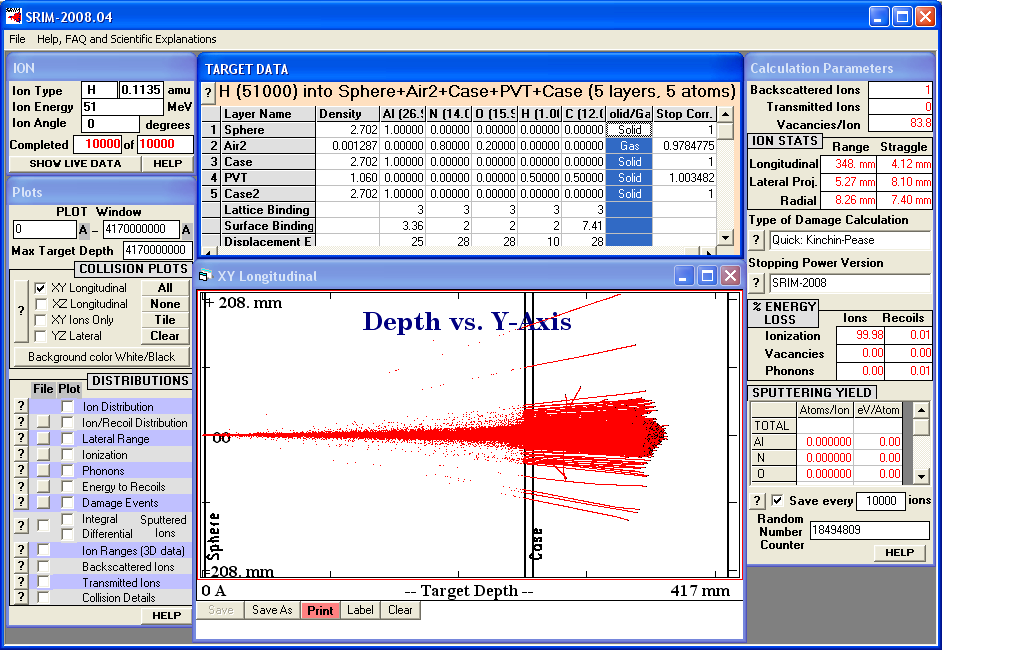
\includegraphics[width=6in]{TRIM_TeachSpin.PNG}
\end{figure}
These numbers are at odds with the stopping power claimed in the Teachspin documentation,
which is 120 MeV/c in one place and 180 MeV/c in another.
These higher numbers may be for vertical muon entry, which I did not model.


\newpage
\begin{thebibliography}{10}

\bibitem{Apsel1978}
D. Apsel,
"Gravitational, electromagnetic, and nuclear theory ",
{\em 	International Journal of Theoretical Physics} v.17 \#8 643-649 (Aug 1978)
DOI: 	10.1007/BF00673015

\bibitem{Apsel1979}
D. Apsel,
"Gravitation and electromagnetism",
{\em General Relativity and Gravitation} v.10 \#4 297-306 (Mar 1979)
DOI: 10.1007/BF00759487

\bibitem{Apsel1981}
D. Apsel,
"Time dilations in bound muon decay",
{\em General Relativity and Gravitation} v.13 \#6 605-607 (Jun 1981)
DOI: 10.1007/BF00757247

\bibitem{Landman2012}
H. Landman,
"An Elementary Approach to Quantum Time Dilation",
\url{http://www.riverrock.org/~howard/QuantumTime21.pdf}
An earlier version of this was posted to the Arxiv server but immediately removed by site administrators.

\bibitem{Coan2006}
T. Coan, T. Liu, J. Ye,
"A Compact Apparatus for Muon Lifetime Measurement and Time Dilation Demonstration in the Undergraduate Laboratory",
{\em Am.J.Phys.} 74, 161-164 (2006)  arXiv:physics/0502103v1

\bibitem{Teachspin}
\url{http://www.teachspin.com/instruments/muon_physics/}

\bibitem{SRIM}
\url{http://www.srim.org}

\bibitem{CaltechMuon}
"Lifetime of the muon",
Physics 77 experiment 15 handout,
Caltech (Sep 2000)
\url{http:www.pma.caltech.edu/~ph77/labs/exp15.pdf}

\bibitem{Berkeley2012}
"Muon Lifetime",
Physics 111 wiki, U C Berkeley,
\url{http://labs.physics.berkeley.edu/mediawiki/index.php/Muon_Lifetime}

\bibitem{Akerlof2009}
C.~W. Akerlof,
"Measurement of the Muon Lifetime",
\url{https://instructor.physics.lsa.umich.edu/adv-labs/Muon_Lifetime/MuonLifetime.pdf}

\bibitem{Hansen2001}
A. Hansen,
"Measurement of Muon Lifetime and Mass Using Cosmic Ray Showers",
Physics 4052 report, U. Minnesota (4 May 2001),
\url{http://mxp.physics.umn.edu/s01/Projects/Muon/muonfinal1c.pdf}

\bibitem{CRDetectors}
"Cosmic Ray Muon Detectors: Particle Physics Using Nature's Accelerator"
\url{http://quarknet.fnal.gov/toolkits/new/crdetectors.html}

\bibitem{FermiLabDetector}
"QuarkNetter Reports: The Fermilab Detector",
\url{http://quarknet.fnal.gov/toolkits/new/fnaldet.html}

\bibitem{wiki_exponential}
\url{http://en.wikipedia.org/wiki/Exponential_distribution}

\bibitem{Gold2007}
J.~I. Gold \& M.~N. Shadlen,
"The Neural Basis of Decision Making",
{\em Annu. Rev. Neurosci.} 30:535�74 (2007)
doi: 10.1146/annurev.neuro.29.051605.113038

\bibitem{Sayyad1969}
G.~M. El-Sayyad,
"Information and Sampling from the Exponential Distribution",
{\em Technometrics}
v.11 \#1 41-45 (Feb 1969)

\bibitem{Al-Athari2008}
F.M. Al-Athari,
"Estimation of the Mean of Truncated Exponential Distribution",
{\em Journal of Mathematics and Statistics} 4(4) 284-288 (2008)

\bibitem{wikiUniform}
\url{http://en.wikipedia.org/wiki/Uniform_distribution_(continuous)}

\bibitem{MuLan2007}
MuLan Collaboration (Chitwood et al.),
"Improved Measurement of the Positive Muon Lifetime and Determination of the Fermi Constant",
{\em Phys. Rev. Lett.} 99:032001, (2007),
arXiv:0704.1981. Bibcode 2007PhRvL..99c2001C,
doi:10.1103/PhysRevLett.99.032001

\bibitem{Becker2003}
W. Becker \& A. Bergmann,
"Detectors for High-Speed Photon Counting", (2003)
\url{http://www.boselec.com/products/documents/FastDetectorsandSources.pdf}
or
\url{http://www.scribd.com/doc/15722917/85/Transit-Time-Spread}

\bibitem{GNUOctave}
\url{http://www.gnu.org/software/octave/}

\bibitem{wikiOctave}
\url{http://en.wikipedia.org/wiki/GNU_Octave}

%\bibitem{wikiAl}
%\url{http://en.wikipedia.org/wiki/Isotopes_of_aluminium}

%\bibitem{wikiMg}
%\url{http://en.wikipedia.org/wiki/Isotopes_of_magnesium}

%\bibitem{Kontopidis2011}
%\url{http://gkontopidis.com/blog/2011/tera-ohm-divider-2/}

%\bibitem{Monroe285}
%\url{http://www.monroe-electronics.com/esd_pages/esd_instrumrnts.htm}

%\bibitem{PGP3121}
%\url{http://www.pgpelectronics.com/Products/DCNA.htm}

%\bibitem{AlphaLab}
%\url{http://www.trifield.com/content/ultra-stable-surface-dc-volt-meter/}

%\bibitem{MissionInst}
%\url{http://www.missioninstruments.com}

%\bibitem{Monroe282M}
%\url{http://www.monroe-electronics.com/esd_pages/fieldmeters.htm#282m}

%\bibitem{SimcoIon}
%\url{http://www.simco-ion.com/IndustrialProducts/InstrumentationMetering/FMX003ElectrostaticFieldmeter.aspx}

%\bibitem{ETS222}
%\url{http://www.electrotechsystems.com/Products.aspx?ProdID=170946}

%\bibitem{MacDonald2002}
%R.P. MacDonald,
%"Examination And Removal Of Backgrounds For Twist At Triumf",
%master's thesis Alberta U. (2002) 

%\bibitem{Marshall:1991wb} 
 %G.~M.~Marshall,
%``Muon beams and facilities at Triumf,''
%Z.\ Phys.\ C {\bf 56}, S226 (1992).
%%CITATION = ZEPYA,C56,S226;%%
  
%\bibitem{TRIUMFwiki}
%\url{http://www.triumf.info/wiki/tug/index.php/Users\%27_Handbook}
  
%\bibitem{MTW}
%Misner, Thorne, Wheeler,
%{\em Gravitation}

%\bibitem{deBroglie1925}
%L. de Broglie,
%{\em Recherches sur la Th\'{e}orie des Quanta} (1925),
%translated by A.F. Kracklauer as
%{\em On the Theory of Quanta} (2004)
%\url{http://www.ensmp.fr/aflb/LDB-oeuvres/De_Broglie_Kracklauer.pdf}

%\bibitem{Hestenes2008}
%D. Hestenes, "Electron time, mass and zitter" (2008)
%\url{http://www.fqxi.org/data/essay-contest-files/Hestenes_Electron_time_essa.pdf}

%\bibitem{Schrodinger1925}
%E. Schr\"{o}dinger, letter to W. Wien (27 Dec 1925)

%\bibitem{Rodrigues1983}
%W.A. Rodrigues Jr.,
%"The Standard of Length in the Theory of Relativity and Ehrenfest Paradox",
%{\em Il Nuovo Cimento} v.74 B \#2 199-211 (11 April 1983)

%\bibitem{Ryff1985}
%L.C.B. Ryff,
%"The Lifetime of an Elementary Particle in a Field",
%{\em General Relativity and Gravitation} v.17 \#6 515-519 (1985)

%\bibitem{Beil1987}
%R.G. Beil,
%"Electrodynamics from a Metric",
%{\em Int. J. of Theoretical Physics} v.26 \#2 189-197 (1987)

%\bibitem{vanHolten1991}
%J.W. van Holten,
%"Relativistic Time Dilation in an External Field",
%NIKHEF-H/91-05 (1991)

%\bibitem{vanHolten1993}
%J.W. van Holten,
%"Relativistic Dynamics of Spin in Strong External Fields",
%\url{arXiv:hep-th/9303124v1}, (24 March 1993)

%\bibitem{Hwang2002}
%W. Y. Hwang, D. Ahn, S. W. Hwang, Y. D. Han,
%"Entangled quantum clocks for measuring proper-time difference",
%{\em Eur. Phys. J. D,} v.19 \#1, 129-132 (April 2002)  DOI:10.1140/epjd/e20020065

%\bibitem{Creator2004}
%"time dilation in an electromagnetic potential" (2004)\\
%\url{http://www.physicsforums.com/archive/index.php/t-57510.html}

%\bibitem{Duda2010}
%\url{http://groups.google.com/group/sci.physics.relativity/browse_thread/thread/3be6a489686aed86/}

%\bibitem{Heaviside1893}
% O. Heaviside,
% "A gravitational and electromagnetic analogy",
%The Electrician 31: 81�82 (1893)

%\bibitem{Jefimenko1992}
%O.D. Jefimenko,
%{\em Causality, electromagnetic induction, and gravitation: a different approach to the theory of electromagnetic and gravitational fields},
%Electret Scientific (1992)

%\bibitem{Einstein1907}
%A. Einstein, "\"{U}ber das Relativit\"{a}tsprinzip und die aus demselben gezogenenn Folgerungen",
%{\em Jahrbuch der Radioaktivit\"{a}t und Elektronik} 4, 411-462 (1907);
%English translation, "On the relativity principle and the conclusions drawn from it",
%{\em The Collected Papers}, v.2, 433-484 (1989)

%\bibitem{Schwartz1977}
%H.M. Schwartz, "Einstein's comprehensive 1907 essay on relativity, part 1",
%{\em Am. J. Physics} 45, 512-517 (1977)

%\bibitem{Jammer2006}
%M. Jammer, {\em Concepts of Simultaneity: from Antiquity to Einstein and Beyond}, Johns Hopkins U. Press (2006)

%\bibitem{Soler2006}
%D. Soler.
%"Rigid Motions in Relativity: Applications",
%in L. Momas, J.Diaz Alonso (eds.),
%{\em A Century of Relativity Physics} 611-614, AIP (2006)

%\bibitem{Klauber1998}
%R. Klauber,
%"New Perspectives on the Relativistically Rotating Disk and Non-time-orthogonal Reference Frames",
%{\em Found. Phys. Lett.} v.11 405-443 (1998)
%gr-qc/0103076

%\bibitem{Farnham1995}
%D.L. Farnham, R.S. Van Dyck, Jr., P.B. Schwinberg,
%"Determination of the Electron's Atomic Mass and the Proton/Electron Mass Ratio via Penning Trap Mass Spectroscopy",
%{\em Phys. Rev. Lett.} 75, 3598 - 3601 (1995)
%\url{http://link.aps.org/doi/10.1103/PhysRevLett.75.3598}
%%DOI: 10.1103/PhysRevLett.75.3598

%\bibitem{Natarajan1993}
%V. Natarajan,
%"Penning trap mass spectroscopy at 0.1 ppb",
%M.I.T. PhD thesis (1993)
%\url{http://dspace.mit.edu/handle/1721.1/28017}

%\bibitem{VanDyck2009}
%R.S. Van Dyck, Jr., personal communications, June 2009

%\bibitem{Swartz2003}
%C. Swartz,
%{\em Back-Of-The-Envelope Physics}, p. 78
%(2003)

%\bibitem{Millikan1910}
%R.A. Millikan,
%"A new modification of the cloud method of determining the elementary electrical charge and the most probable value of that charge",
%{\em Phys. Mag.} XIX 6, 209 (1910)

%\bibitem{Millikan1913}
%R.A. Millikan,
%"On the Elementary Electric charge and the Avogadro Constant",
%{\em Phys. Rev.} II 2, 109 (1913)

%\bibitem{wiki_oil}
%\url{http://en.wikipedia.org/wiki/Oil-drop_experiment}

%\bibitem{Tjoelker1990}
%R.L. Tjoelker,
%{\em Antiprotons in a Penning Trap: A New Measurement of the Inertial Mass},
%PhD thesis, Harvard U., 1990
%\url{http://hussle.harvard.edu/~gabrielse/gabrielse/papers/1990/1990_tjoelker/}

%\bibitem{Hori2006}
%M. Hori et al.,
%"Determination of the Antiproton-to-Electron Mass Ratio by Precision Laser Spectroscopy of $\bar{p}$He$^+$",
%{\em Phys. Rev. Lett.} 96, 243401 (2006)
%\url{http://link.aps.org/doi/10.1103/PhysRevLett.96.243401}
%DOI: 	10.1103/PhysRevLett.96.243401

%\bibitem{Hayano2007}
%R.S. Hayano, M. Hori, D. Horv\'{a}th, E. Widmann,
%"Antiprotonic helium and CPT invariance",
%{\em Rep. Prog. Phys.} 70 1995�2065 (2007)
%\url{http://asacusa.web.cern.ch/ASACUSA/home/publications/rpp7_12_R01.pdf}
%DOI: 10.1088/0034-4885/70/12/R01

%\bibitem{Horvath2008}
%D. Horv\'{a}th,
%"Antiprotonic helium and {\em CPT} invariance",
%2008

%\bibitem{Wheeler1947}
%J.A. Wheeler,
%"Mechanism of Capture of Slow Mesons",
%{\em Phys. Rev.} 71 320 (1947)

%\bibitem{Andreev2007}
%V.A. Andreev et al.,
%"Measurement of the Rate of Muon Capture in Hydrogen Gas and 
%Determination of the Proton�s Pseudoscalar Coupling $g_P$",
%submitted to Phys.Rev.Lett
%arXiv:0704.2072v1 [nucl-ex]

%\bibitem{Kammel2003}
%P.Kammel,
%"Muon Capture and Muon Lifetime",
%arXiv:nucl-ex/0304019v2

%\bibitem{Bell1955}
%J.P. Bell,
%in K. Siegbahn (ed.),
%{\em Beta- and Gamma-Ray Spectroscopy},
%Interscience (1955)

%\bibitem{Aharonov1959}
%Y. Aharonov, D. Bohm,
%"Significance of Electromagnetic Potentials in the Quantum Theory",
%{\em Phys. Rev.} 115, 485-491 (1959). 
%\url{http://link.aps.org/doi/10.1103/PhysRev.115.485}
%DOI: 10.1103/PhysRev.115.485

%\bibitem{Ehrenberg1949}
%W. Ehrenberg, R. E. Siday,.
%"The Refractive Index in Electron Optics and the Principles of Dynamics",
%{\em Proc. Phys. Soc.} B62: 8-21 (1949).
%DOI: 10.1088/0370-1301/62/1/303

%\bibitem{Allman}
%B.E. Allman, A. Cimmino, A.G. Klein,
%Reply to "Comment on �Quantum Phase Shift Caused by Spatial Confinement" by Murray Peshkin,
%{\em Foundations of Physics} v.29 \#3 325-332 (March 1999). DOI:10.1023/A:1018858630047

%\bibitem{Chitwood2007}
%D.B. Chitwood et al. (MuLan Collaboration),
%"Improved Measurement of the Positive Muon Lifetime and Determination of the Fermi Constant",
%{\em Phys. Rev. Lett.} 99:032001(2007)
%DOI: 	10.1103/PhysRevLett.99.032001
%arXiv:0704.1981v2 [hep-ex]

%\bibitem{Bennett2004}
%G.W. Bennett et al.,
%"Measurement of the Negative Muon Anomalous Magnetic Moment to 0.7 ppm",
%{\em Physical Review Letters} 92; 1618102 (2004).  arXiv:hep-ex/0401008 v3 (21 Feb 2004)

%\bibitem{Eaton1999}
%G.H. Eaton, S.H. Kilcoyne,
%"Muon Production: Past, Present, and Future",
%in S.L. Lee et al. (eds), {\em Muon Science: Muons in Physics, Chemistry and Materials} 11-37, (1999)

%\bibitem{Heffner1984}
%R.H. Heffner,
%{\em Muon sources for solid-state research},
%National Academy Press (1984)

%\bibitem{Kuno2001}
%Y. Kuno, Y. Okada, "Muon decay and physics beyond the standard model",
%{\em Rev. Mod. Physics} 73 151-202 (Jan 2001)

%\bibitem{Ritbergen1999}
%T. van Ritbergen, R.G. Stuart,
%"Complete 2-Loop Quantum Electrodynamic Contributions to the Muon Lifetime in the Fermi Model",
%{\em Phys. Rev. Lett.} 82, 488-491 (1999)
%\url{http://link.aps.org/doi/10.1103/PhysRevLett.82.488}
%DOI: 10.1103/PhysRevLett.82.488

%\bibitem{Fermi1947}
%E. Fermi, E. Teller,
%"The Capture of Negative Mesotrons in Matter",
%{\em Physical Review} v.72 \#5 399-408 (1947)

%\bibitem{Tonomura1982}
%A. Tonomura et al.,
%"Observation of Aharonov-Bohm Effect by Electron Holography,"
%{\em Phys. Rev. Lett.} 48 1443-1446 (1982)

%\bibitem{Hughes2001}
%V.W. Hughes,
%"The Muon Anomalous Magnetic Moment", in
%E. Arimondo, P. De Natale, \& M. Inguscio (eds.),
%{\em Atomic Physics 17} (2001)

%\bibitem{Colella1975}
%R. Colella, A. W. Overhauser, S. A. Werner,
%"Observation of Gravitationally Induced Quantum Interference",
%{\em Phys. Rev. Lett.} 34, 1472 (1975)

%\bibitem{Arndt2001}
%M. Arndt, O. Nairz, J. Petschinka, A. Zeilinger, "High Contrast Interference with C$_{60}$ and C$_{70}$",
%{\em C. R. Acad. Sci. Paris}, t.2 S�rie IV, 581-585 (2001)

%\bibitem{Nairz2003}
%O. Nairz, M. Arndt, A. Zeilinger, "Quantum Interference Experiments with Large Molecules",
%{\em American Journal of Physics} 71, 319 (2003)

% for future reference

%\bibitem{Stephani2003}
%H. Stephani et al.,
%{\em Exact solutions of Einstein's field equations} 2nd Ed., Cambridge U. Press (2003)

%\bibitem{MacCallum2006}
%M.A.H. MacCallum,
%"Finding and using exact solutions of the Einstein equations",
%in L. Momas, J.Diaz Alonso (eds.),
%{\em A Century of Relativity Physics} 129-143, AIP (2006)

%\bibitem{Murayama2003}
%H. Murayama,
%"CPT Tests: Kaon vs Neutrinos",
%arXiv:hep-ph/0307127

%\bibitem{Sachs1987}
%R.G. Sachs,
%{\em The Physics of Time Reversal},
%U. Chicago Press (1987),
%p.175

%\bibitem{Czarnecki2000}
%A. Czarnecki, G.P. Lepage, W.J. Marciano,
%"Muonium decay",
%{\em Phys. Rev.} D 61, 073001 (2000)
%\url{http://link.aps.org/doi/10.1103/PhysRevD.61.073001}
%DOI: 10.1103/PhysRevD.61.073001 

% metal sphere fabrication
%
% \url{http://www.helandermetal.com/metal-hemispheres-metal-cones.html}
%
%
% metal mixing bowls
%
% \url{http://www.jesrestaurantequipment.com/mixing-bowl-capacity-188-stainless-steel-mirror-finis-p-740899.html}

\end{thebibliography}

\end{document}